\documentclass{scrartcl}
\usepackage{graphics}
\usepackage{thmtools}
\usepackage{wasysym}
%\usepackage{arxiv}
%\usepackage{enseign}

\usepackage{iftex}                      % check which engine is compiling this file
\iftutex                                % xelatex or lualatex specific first
 % \usepackage{fontspec}                % font selection in xelatex/lualatex
 \defaultfontfeatures {Ligatures=TeX}
 \usepackage{unicode-math}              % amssymb,amsmath eq, to show $θ$ as θ
 \unimathsetup{math-style=TeX}
 \setmathfont{Stix Two Math}
 \ifLuaTeX
  %  \usepackage{luatex85}              % compatibility of luatex with xy
   \usepackage{lualatex-math}
 \fi
\else                                   % 8bit (e.g. pdflatex) specific
\usepackage[T1]{fontenc}                % use 8-bit T1 fonts
%\usepackage[utf8]{inputenc}       % allow utf-8 input, for texlive-2016 and older
\fi
\usepackage{alphabeta}              % in LuaLaTeX use {unicode-math}

\usepackage{amsthm}
\usepackage{amsbsy,amsmath,amssymb,amscd,amsfonts}
\usepackage[pagebackref=true]{hyperref}
\usepackage[nameinlink,capitalize,noabbrev]{cleveref}
%\usepackage{hyperref}
%\usepackage{url}            % simple URL typesetting
%\usepackage{booktabs}       % professional-quality tables
%\usepackage{nicefrac}       % compact symbols for 1/2, etc.
%\usepackage{microtype}      % microtypography

\usepackage{graphicx,float,latexsym,color}
%\usepackage{refcheck}
%\usepackage{mathspec}
\usepackage[font={scriptsize,it}]{caption}
\usepackage{subcaption}
%\let\proof\relax
%\let\endproof\relax

\usepackage{makecell}

% usar \defcommand em vez de \newcommand ou \renewcommand
% funciona como \def em tex - vai definir, se ainda não definida,
% se já definida, vai redefinir
\makeatletter\def\defcommand{\@ifstar\defcommand@S\defcommand@N} \def\defcommand@S#1{\let#1\outer\renewcommand*#1} \def\defcommand@N#1{\let#1\outer\renewcommand#1} \makeatother

\renewcommand{\arraystretch}{1.2}

\usepackage[dvipsnames]{xcolor}

\newtheorem{theorem}{Theorem}
\newtheorem*{theorem*}{Theorem}
\newtheorem{observation}{Observation}
\newtheorem{proposition}{Proposition}
\newtheorem{conjecture}{Conjecture}
\newtheorem{corollary}{Corollary}
\newtheorem{lemma}{Lemma}
\theoremstyle{remark}
\newtheorem{remark}{Remark}
\theoremstyle{definition}
\newtheorem{definition}{Definition}
\newtheorem{question}{Question}
\hypersetup{
    %bookmarks=true,         % show bookmarks bar?
    %unicode=true,          % non-Latin characters in Acrobat’s bookmarks
    pdftoolbar=true,        % show Acrobat’s toolbar?
    pdfmenubar=true,        % show Acrobat’s menu?
    pdffitwindow=false,     % window fit to page when opened
    pdfstartview={FitH},    % fits the width of 
    colorlinks=true,       % false: boxed links; true: colored links
    linkcolor=OliveGreen,          % color of internal links (change box color with linkbordercolor)
    citecolor=blue,        % color of links to bibliography
    filecolor=black,      % color of file links
    urlcolor=red           % color of external links
}

\usepackage{lineno}
\def\linenumberfont{\normalfont\small\sffamily}
%a4: 210 x 297
%\textwidth=125mm
%\textheight=195mm
\arraycolsep=2pt
\captionsetup{width=120mm}

 \newcommand{\Mod}[1]{\ (\mathrm{mod}\ #1)}
 
\usepackage{comment}
\usepackage{microtype}
\usepackage{footnote}
%\usepackage{tablefootnote}
%\usepackage{longtable}

%\usepackage{night}

\newcommand{\E}{\mathcal{E}}
\newcommand{\T}{\mathcal{T}}
%\newcommand{\C}{\mathcal{C}}
\defcommand{\C}{\mathcal{C}}
\newcommand{\F}{\mathcal{F}}
\renewcommand{\P}{\mathcal{P}}
\newcommand{\D}{\mathbb{D}}
\renewcommand{\T}{\mathbb{T}}
\newcommand{\R}{\mathbb{R}}
\newcommand{\Cp}{\mathbb{C}}
\newcommand{\ol}{\overline}
\renewcommand{\l}{\lambda}
\newcommand{\X}{\mathcal{X}}

\newcommand{\torp}[2]{\texorpdfstring{#1}{#2}}
\newcommand{\ab}{_{\alpha,\beta}}

\date{\today}
\author{Sergey Galkin, Ronaldo Garcia, Dan Reznik}
\begin{document}
\title{On Affine Images of Regular Polygons}
\maketitle



\begin{abstract}
We describe and prove two new invariants manifested by the ``homothetic'' family, i.e., a family of Poncelet N-gons interscribed between two concentric, axis-aligned, homothetic ellipses. In contradistinction with the confocal family (elliptic billiard) which conserves perimeter, Joachimsthal's constant, and the sum of internal angle cosines, the homothetic family conserves area, sum of squared sidelengths, and the sum of internal angle cotangents.
\end{abstract}


\tableofcontents

\section{Introduction}
\label{sec:intro}
% 

Let $\FF$ be a family of affine images of a regular polygon
whose circumcircle is sent to an ellipse with fixed semi-axes of length $a,b$.

Let us say that a \emph{trace} of a ''quantity'' is the arithmetic mean of its values on the vertices of the polygon in $\FF$.
A priori the trace depends on the chosen polygon and/or on the particular transformation $T\in\FF$.
We will explicitly compute the traces of the ''interesting'' quantities below.
In particular, we prove that these are constant over $\FF$
and compute their limits for infinite gonality (denoted further by $N$):

\begin{itemize} \itemsep0em
    \item \eqref{:norm2}: the squared distance to any fixed point; see \cref{fig:homot_norm}.
    \item \eqref{:sqr_si}: the squared sidelength.
    \item \eqref{:cot}: the cotangent of an internal angle.
    \item \eqref{:dist-focus}: the distance to a focus of $\EE$.
    \item \eqref{:kappa}: \textcolor{magenta}{the kinetic energy} $\kappa^{-2/3}$, where $\kappa$ is the curvature of the ellipse $\EE$.
    \item \eqref{:ell2}: the squared sidelength of the evolute polygon (except squares and hexagons). 
    \item \eqref{:as}: the signed area of the evolute polygon (except squares).
\footnote{We explain later in which sense area can be thought as a function.}
\end{itemize}

As a part of the computation
we verify that each of the traced quantities is a Laurent polynomial
when expressed in terms of the natural coordinate on the circle.
Then the application of \cref{:Laurent}
implies that its trace is constant for all gonality higher than the degree of the polynomial,
and the remaining traces are explicitly computed in terms of coefficients by \cref{:fourier-of-trace}. The degree for each Laurent polynomial appears on \cref{tab:invariants-degrees}.

\subsection*{Article organization}
We start from \cref{sec:polygonomials}
by defining the polygons and (functions on) their moduli spaces,
and explaining our selection criteria
for the ''quantity'' to be ''interesting''.
After this section it will be clear why the kinetic energy
is considered to be an interesting quantity,
but coordinates and momenta (whose traces are also constant) are not:
the former is invariant with respect to the Euclidean transformation group,
while the latter are covariant (equivariant).

In \cref{sec:trigo}
we give trigonometric preliminaries,
then introduce the traces
in \cref{sec:traces},
and characterize functions with constant trace
by \cref{:fourier-of-trace,:functoriality,:Laurent,:characterization,:strange,:ergodic},
from which all the remaining claims follow by straightforward computations,
which are described in \cref{sec:examples}.
In \eqref{sec:areas} we discuss oriented areas,
many natural oriented areas are constant even before the tracing,
and also we explain how they split into local summands.
In \eqref{sec:scalar} we discuss functions that are quadratic polynomials for obvious reasons --- scalar products of linear transformations.
In \eqref{sec:cot} we discuss cotangents that also turn out to be quadratic.
In \eqref{sec:focuspocus} we show that distance to the focus is linear
and $κ^{-2/3}$ is quadratic: a priori we knew only that their square and cube are polynomials,
but these polynomials turned out to be
a perfect square (of a coordinate)
and a perfect cube (of the kinetic energy).
In \eqref{sec:evolute} we compute the quantities
associated with evolute polygons (of degrees four and six)
using an explicit parametrization
for the evolute\footnote{The curve sweeped by centers of curvature (centers of the oscullating circles).},
of the ellipse, a curve affinely equivalent to the \href{https://en.wikipedia.org/wiki/Astroid}{astroid}
\footnote{Plane algebraic curve $x^{2/3}+y^{2/3}=1$,
see e.g. \url{https://en.wikipedia.org/wiki/Astroid},
\url{https://mathshistory.st-andrews.ac.uk/Curves/Astroid},
\url{http://xahlee.info/SpecialPlaneCurves_dir/Astroid_dir/astroid.html}}.

In \cref{sec:video-table} we (i) 
list the polynomial quantities sorted by their degrees
and hypothesize on what could be their ``analogues'' in the elliptic billiard
and (ii) provide a list of illustrative videos of the phenomena herein.
For convenience, all used symbols appear in \cref{app:symbols}.





\section{Polygonomials}
\label{sec:polygonomials}
In this section we define polygons,
their moduli spaces,
and various classes of functions on these spaces
(polygonomials, ratiogonal functions, etc).

%   polygonomial  = polynomial on polygon space, (+ G-invariant?)
%   ratiogonal    = ratio of polygonomials

Let $F$ be a principal homogeneous space (a torsor) over a group $E$.
In our main examples either $F$ will be an affine space over a vector space $E$,
of $F$ will be a torsor over a semi-abelian variety $E$
(e.g. $F$ will be a curve of arithmetic genus one and $E$ will be its generalized Jacobian),
but so far any $E$ (even non-abelian) would suffice,
however we will use additive notation $(+,-,0)$ for the operations on $E$
and action $E:F$ to reserve the multiplicative notation for the action
of another group $G$ to be defined shortly later.


\begin{definition} \label{d:marked-f-polygon}
For $n\geq 0$ define \emph{a marked ($F$-)polygon}
to be a map $P : \Z/n \to F$,
so that $P(i), i \in \Z/n$ is a set of points in $F$,
that we interpret as the vertices.
The number $n$ will be called
\emph{gonality}
\footnote{A relation with gonality of algebraic curves will be explained shortly.},
so $P$ will be called an $n$-gon.
\footnote{Except for the case $n=0$ when we call it an $\infty$-gon
(abusing notation, gonality zero is the same as gonality infinity).
Note that so far it would suffice to consider only $\infty$-gons
and defining $n$-gons as $\infty$-gons with the map $P$ being $n$-periodic.}
\end{definition}

One constructs \emph{oriented sides} $e(i) \in E$ as the (right) differences

\begin{equation} \label{eq:P2e}
P(i) = P(i-1) + e(i)
\end{equation}

For $n>0$ the vectors $e(1),...,e(n)$ satisfy a relation

\begin{equation} \label{eq:zerosum}
  e(1) + e(2) + ... + e(n) = 0       
\end{equation}

Two polygons $Q,P$ have equal associated side-vectors
if and only if they differ by a (left) translation,
i.e. exists a $t \in E$ such that for all $i$
\begin{equation} \label{eq:left-translation}
Q(i) = t + P(i)
\end{equation}

The polygons that differ by a (left) translation
are called ($E$-)equivalent,
and the space of the ($F$-)polygons up to a (left) translation
is the (left) quotient $E \backslash F^n$.

\begin{definition} \label{d:marked-e-polygon}
\emph{A marked $E$-polygon}
is a collection of $n$ elements of $E$ subject
to the condition \eqref{eq:zerosum}.
\end{definition}

\begin{remark} \label{rem:twist}
Analogously one defines for any $τ\in E$ the \emph{$τ$-twisted ($E$-)polygons}
by replacing $0$ in the right hand side of \Cref{eq:zerosum} by $τ$.
Similarly, \emph{$τ$-twisted ($F$-)polygons} are given by
quasi-periodic functions $P : \Z \to F$, i.e.
\begin{equation} \label{eq:twisted-f-polygon}
P(i) = P(i-n) + τ
\end{equation}
\end{remark}

By a convenient abuse of notation
(that happens only for non-trivial $E$-torsors $F$)
we make no further distinction between $E$-equivalence classes of $F$-polygons
and $E$-polygons.

\begin{definition} \label{d:poncelet-polygon}
A marked/oriented/unoriented ($E$- or $F$-)polygon is called
\emph{Poncelet ($E$- or $F$-)polygon}
if the function $e$ is constant. Clearly Poncelet $\infty$-gons
are classified by vectors of $E$, and Poncelet $n$-gons for $n\geq 1$
are classified by $n$-torsion vectors $e \in E[n]$.
\end{definition}

Note that the cyclic group acts on the space of the marked polygons by shifting the marking
$s P(i) = P(i+1)$, and later (after setting up the moduli space of marked polygons)
by an \emph{oriented polygon} we would mean a $\Z$-equivalence class of the polygons.
Similarly an \emph{unoriented polygon} is an equivalence class of polygons with respect to the dihedral group,
generated by the shifts of the cyclic group and a reflection $r P(i) = P(-i)$.

For $0<n<\infty$ given any $(n-1)$ vector-sides $e(i)$
the remaining one is uniquely determined by \eqref{eq:zerosum},
thus the space of all marked $n$-gons in $E$ can be identified
with $(n-1)$-st Cartesian power of $E$,
denoted as $E^{\times (n-1)}$ or $E^{n-1}$.
Consider the space of (polynomial/rational) functions on $E^{n-1}$.

Further endow $E$ with an action of a group $G$ by group homomorphisms of $E$.
\begin{example} \label{ex:G:E}
\begin{itemize}
\item $E$ is a vector space $V$ with a symmetric bilinear form $B$ and $G = \SO(V,B)$
a special orthogonal group
\item $E$ is a complex vector space $V$ with a sesquilinear form $B$ and $G = \Un(V,B)$
a unitary group
\item $E=V$ is same as above, but group $G$ is extended by homotheties $v\mapsto λ v$
% \item $E$ an elliptic curve and $G$ generated by involution $e\mapsto -e$
\end{itemize}
\end{example}

The group $G$ acts (diagonally) on the spaces of polygons: for all $g \in G$
\begin{equation} \label{eq:action}
(e(1),...,e(n)) = e \mapsto  g e := (g e(1), ..., g e(n))
\end{equation}

and gives an equivalence relation thereon ($G$-equivalence).
In the case of twisted polygons (\cref{rem:twist}) the group $G$ also acts on
the twists $t$.

We would like to "identify" $G$-equivalent polygons in order to consider
moduli spaces of $G:E$-polygons, whose points are (some) orbits of this action.

Thus polynomial/rational functions on the moduli space of $G:E$-$n$-gons are defined
as $G$-invariant polynomial/rational functions on $E^{n-1}$.

Let us call them ($G$-)polygonomials and ($G$-)ratiogonal functions, respectively.

The case $n=2$ corresponds to $G$-invariant functions on $E$,
and in our situation typically there won't be that many non-constant invariants:
\begin{example} \label{ex:B11}
In \Cref{ex:G:E} the ring of invariants with respect to $\SO$ or $\Un$
is $\k[B_{11}]$, the ring of polynomials freely generated by $B_{11} := B(e_1,e_1)$.
The generator is not invariant with respect to the homotheties,
but has grading $2$.
\end{example}
In what follows let us localize to $e(i)\neq0$, so that
$G$-invariants $B_{ii}$ from example \Cref{ex:B11} are non-zero/invertible.

The extra grading with respect to the homotheties is useful,
and typically for geometric invariant theory, we will consider a bigger group
$G^* \supset G$ and its character $χ : G^* \to \C^*$
such that $G = \Ker χ$. Then instead of $G$-invariants we consider
quasi-invariants with respect to tensor powers of $χ$:
\begin{equation}
\oplus_{k\in\Z} \k[E^{n-1}]^{kχ}
\end{equation}

Every map $f: E^{n-1}\to E$ can be used to pull back the quasi-invariants
$f^*: \k[E]^{kχ} \to \k[E^{n-1}]^{kχ}$.

\begin{example}
In \Cref{ex:G:E} natural $G$-invariants on $E^2$ are tautologically
given by the pairings $B_{ij} := B(e_i,e_j)$ for $i,j\in \Z/n$.
Functions $B_{ij}$ satisfy linear relations
\begin{equation}
\sum_i B_{ij} = 0 = \sum_j B_{ij}
\end{equation}
and $B_{ij} = B_{ji}$ (resp. $B_{ij} = \ol{B_{ji}}$),
so only $\frac{n(n-1)}{2}$ of them are linearly independent.
\end{example}

Let us see the $G$-invariants of $E$-triangles
(equivalently, $G$-invariants of a pair of vectors in $E$).

\begin{example}
There are three quasi-invariants with character $χ$,
and the field of invariants is freely generated by their two ratios.
Indeed, if $e_2$ lies in a complex line spanned by non-zero $e_1$
there is a unique element of $\tilde{G}$ that maps $e_1$ to $1\in \C$.
Then the real and imaginary coordinates of the image of $e_2$ (i.e. of $e_2/e_1$)
are the free generators of the field of invariants.
Their ratio is the (co)tangent of the angle between vector-sides $e_1$ and $e_2$
of the triangle, multiplied by $-1$.
\end{example}




\section{Poncelet configurations}
\label{sec:poncelet}
% Explain Poncelet configuration space
% and the map from the elliptic curve to the moduli space of polygons


\section{Trigonometry}
\label{sec:trigo}

Let $i$ denote imaginary root of unity, so that $i^2=-1$.
Since de Moivre a rotation of a unit circle 
\begin{equation}
S^1 = \{(r,\varphi):r=1\} = \{(x,y): x^2+y^2=1\} = \{z: |z|=1\}
\end{equation}
can be parameterized
either (i) by its angle $\varphi$,
   or (ii) by a pair of Cartesian co-ordinates $(x,y)$ such that $x^2+y^2=1$,
  or (iii) by a unit complex number $z$,
and the parameterizations are related to each other
and to trigonometric functions $\cos,\sin$ by formulae: 
\begin{gather}
\label{eq:demoivre}
z = x + y \cdot i \qquad = \exp(i \varphi) = \cos(\varphi) + \sin(\varphi) \cdot i, \\
\label{eq:demoivre2}
\cos(\varphi) = (z+z^{-1})/2 = x, \qquad \sin(\varphi) = (z-z^{-1})/(2i) = y.
\end{gather}
Fixing a reference point $P_0$ one can identify a rotation $\rho$
with a point $\rho(P_0)$.
Thus the composition of rotations as well as the action of a rotation on a point
are described by multiplication of complex numbers.
In particular the rotation $ρ$ by a fixed angle $α = \arg ζ$ is a linear transformation
either in complex co-ordinate 
\begin{equation}
\label{eq:dynamics-complex}
ρ : z\mapsto ζ\cdot z
\end{equation}
or in the real co-ordinates $x,y$
(note that $\bar{ρ(z)} = \bar{ζ}\cdot\bar{z}$ is linear in $\bar{z}$ and $z^{-1} = \bar{z}$ on $S^1$,
so the transformations \cref{eq:demoivre,eq:demoivre2} restricted to $S^1$ are linear).
Also, the sequence of points $\dots,P_{k-1},P_k,P_{k+1},\dots$
is obtained by consecutive fixed rotations $ρ$ (i.e. $P_{k+1} = ρ P_k$ for some $ρ$)
if and only if the corresponding sequence of complex numbers
is a geometric progression:
\[ P_k^2 = P_{k-1} \cdot P_{k+1}. \]

Define a scalar product of two complex-valued functions on the circle by
$(f,g) := \int_{S^1} f \cdot \ol{g} \, dμ_L$, where
$dμ_L$ is the Lebesgue measure
$dμ_L = \frac{d\varphi}{2\pi} = \frac{1}{2πi} \frac{dz}{z}$. 
Laurent monomials form an orthonormal basis
in the Hilbert space $L^2(S^1,\C)$ of functions $f$ with $(f,f)<\infty$,
i.e. any such function has a unique Fourier series
\[ f(z) = \sum_{m\in\Z} \widehat{f}(m) z^m, \]
with Fourier coefficients $\widehat{f}(m) = (f,z^m) = \int_{S^1} f(z) z^{-m} dμ_L$.
A Slightly less convenient orthonormal basis for $L^2(S^1)$ is given by the functions
$1,x_1,y_1,x_2,y_2,\dots$ where $x_n := \Re{z^n} = \frac{z^n+z^{-n}}2 = \cos(n\varphi)$
and $y_n := \Im{z^n} = \frac{z^n - z^{-n}}{2i} = \sin(n\varphi)$.
Its main advantage is that $x_n,y_n$ take real values on $S^1$,
so they form a real basis for the real Hilbert space $L^2(S^1,\R)$. In terms of Fourier coefficients
this real structure is given by $\widehat{f}(-m) = \overline{\widehat{f}(m)}$.
Finally, one can also use a (non-orthogonal) basis $x^n,x^n\cdot y$ ($n\geq 0$),
and the transformation to the basis $x_n,y_n$ is given
by the unique degree-$n$ polynomials $T_n$ (Chebyshëv) and $U_n$ (Kórkin--Zolotarëv)
such that $x_n = T_n(x)$ and $y_{n+1} = y \cdot U_n(x)$.

The reflection $ι$ with respect to the real line is given on a unit circle by
$\varphi\mapsto -\varphi$ or $(x,y)\mapsto (x,-y)$ or $z\mapsto z^{-1} = \bar{z}$.
Any function $f$ on $S^1$ is decomposed into the sum $f = f_+ + f_-$
of a $ι$-invariant (``even'') part $f_+(z) = \frac{f(z)+f(z^-1)}{2}$
and a $ι$-anti-invariant (``odd'') part $f_+(z) = \frac{f(z)-f(z^-1)}{2}$.
The even part is generated by the Joukovsky function $J(z) := x = x_1 = \frac{z+z^{-1}}{2}$
and is naturally isomorphic to the functions on the image: 
(either the unit interval $[-1,1]$, or the affine/projective line, depending on the context).
This is a subalgebra (sum and product of invariant functions is invariant),
and in terms of Fourier coefficients it is given by $\widehat{f}(-m) = \widehat{f}(m)$.
The odd part is a free cyclic module over this algebra
with a generator $y = y_1$,
i.e. any odd function equals to $y$ times a unique even function.

For any bivariate polynomial of degree less than $d$,
the result of the substitution $(x,y) \mapsto (\cos(\varphi),\sin(\varphi))$
can be uniquely written as a linear combination of Laurent monomials $z^k$ 
or $x_k,y_k$ with $|k|<d$,
We will call such elements trigonometric (or Laurent) polynomials of degree less than $d$.
We will further label them ``even'' or ``odd'' if they are invariant or anti-invariant
with respect to the involution $ι$.
An example of an odd rational function which is 
not square-integrable (in particular, not a trigonometric polynomial)
is given by the cotangent:
\begin{equation}
\small
 \label{eq:cotangent}
\cot(\varphi) := \frac{\cos(\varphi)}{\sin(\varphi)} 
= \sum_{n\in\Z} \frac1{\varphi+n\cdotπ}
= i \left(1+\frac{1}{z-1}-\frac{1}{z+1}\right)
% = i \left(1+\frac{2}{z^2-1}  \right) 
= i \frac{z^2+1}{z^2-1} 
=: \xi(z) 
\end{equation}



\section{Traces and Averages}
\label{sec:traces}

Let $ζ$ (resp. $z$) be a complex number associated with a rotation $ρ$ (resp. an initial point $P$),
and $f$ be a function on a circle.
The $L$-step time average with respect to the rotation $ρ$
is a linear operator $T_{L,ζ}$ on the functions of $z$ defined by
\begin{equation} \label{eq:time-average} 
T_{ζ,L} : f \mapsto \frac{1}{L} \sum_{k=0}^{L-1} ρ^{\circ k} f = \frac{1}{L} \sum_{k=0}^{L-1} f(ζ^k \cdot z).
\end{equation}
% if $ζ^N = 1$ we will simply write $\int_{N,z}$.
If $ζ$ is a primitive $N$-th root of unity (in this case define $\ord(ζ)$ to be $N$, otherwise $\infty$)
and $L$ is divisible by $N$
we call the respective sum \emph{the $N$-periodic time average} $T_N[f,z]$,
for generic $L$ note that $\lim_{L\to\infty} T_{ζ,L} f = T_N[f,z]$.
In this case $T_N[f,z] = T_N[f,ζ^k\cdot z]$ for any $k\in\Z$,
so there exists a unique function $T_N f$ (alternatively named $T_ζ f$) of the variable $z_N$,
the \emph{trace}
\footnote{Recall that usually for a map $F: X \to Y$ the trace is an operator that sends $f/X$ to $\tr_F f /Y$ and is defined by
$(\tr_F f) (y) = \sum_{F(x)=y} f(x)$ when it makes sense.
Unlike average, the trace is defined without division by the degree ($N$),
and the average (trace divided by the degree) can be thought as a normalized trace.
For the convenience in this paper we use such normalization,
and further do not distinguish between the trace and the average when both are defined.}
 of $f$ with respect to the map $z\mapsto z^N$,
such that 
\begin{equation} \label{eq:trace}
(T_N f) (z_N \mapsto z^N) = T_N[f,z].
\end{equation}
For example, consideration of \cref{eq:cotangent}
show that the trace of the cotangent $T_N (\cot(\varphi))=T_N(\xi)$ equals 
$\xi(z_N)$ for $N$ even, and $\xi(z_N^2)$ for $N$ odd.
\footnote{Use either explicit rational function of $z$ or Euler's infinite sum.}
%where $ψ = N \varphi$ is the angle co-ordinate on the image. 
The traces $T_N$ (also known as transfers, direct images or push-forwards)
are linear operators on the spaces of functions (differential forms, measures, etc),
and they preserve any of the following properties:
$L^p$ integrability, continuity, smoothness, algebraicity, rationality, Laurent polynomiality.
For $N=0$ the map $z\mapsto z^0$ is constant with the image being a point $z=1$,
so $T_0 f$ makes sense either as a function on a point
or as a generalized function (distribution)
on a circle equal to $\widehat{f}(0)$ times delta-function of the point $z=1$.
When $N$ grows big $T_N f$ approaches $T_\infty f$,
a constant function on $S^1$ equal to $\widehat{f}(0)$.
The trace is functorial: $T_{N_1 \cdot N_2} = T_{N_1} \circ T_{N_2}$
for any pair $N_1,N_2 \in \Z \bigcup \infty$ when $N_1\cdot N_2$ makes sense
(anything but $(0,\infty)$ or $(\infty,0)$).
The functoriality implies
\begin{proposition} \label{:functoriality}
Assume $T_N f$ is constant for some $N$.
Then $T_{N'} f$ is also constant for all $N'$ divisible by $N$,
and the constant equals to the space-average $\widehat{f}(0) = \int_{S^1} f(z) dμ_L$.
\end{proposition}
We will be interested in proving the constancy of $T_N f_N$
for functions $f_N$ that implicitly \emph{depend on $N$},
so instead of the direct application of the proposition
we will have to make this dependence explicit (cf. \cref{:strange})
and decompose $f_N$ into a linear combination
of simpler functions independent of $N$ \cref{:characterization}.

Explicitly, the (non necessarily periodic) time average of
a Laurent monomial $f(z) = c(M) \cdot z^M$ ($M\in\Z$) equals
\begin{equation}
\label{eq:average-monomial}
 \frac{1}{L} \sum_{k=k_0}^{k_0+L-1} c(M) (ζ^k \cdot z)^M
= c(M) z^M \cdot \left( \frac{1}{L} ζ^{M k_0} \sum_{k=0}^{L-1} (ζ^M)^k  \right).
\end{equation}
If $ζ^M=1$ (i.e. if $M$ is divisible by $\ord(ζ)$),
then the second factor equals $1$ and the average equals $c(M) z^M$,
otherwise
\begin{equation} \label{eq:geometric-progression}
\frac{1}{L} \sum_{k=k_0}^{k_0+L-1} c(M) z^M (ζ^M)^k
= \frac{1}{L} \frac{ζ^{M k_0}-ζ^{M(k_0+L)}}{1-ζ^M} c(M) z^M
\end{equation}
by geometric progression formula.
\footnote{The only explicitly computable sum according to Abel.}
In particular, % $N$-periodic time average of 
the trace $T_N c(M) z^M$ is non-zero
if and only if $c(M)\neq 0$ and $M$ is divisible
\footnote{Note that fixed $M$ has but a finite number of integer divisors,
so all $T_N$ of a Laurent polynomial vanish for $N$ higher than the degree,
see \cref{:Laurent}.} 
by $N$,
in fact this is equivalent to the existence of the trace $T_N f$ that satisfies \Cref{eq:trace}.
Let us rephrase it once again:
\begin{equation} \label{:fourier-of-trace}
T_N f = \sum_{m\in\Z} \widehat{f}(N m) z_N^m, \\
\end{equation}
where $z_N$ is the co-ordinate on the image-circle,
related to the co-ordinate on the source-circle by $z_N = z^N$.

In particular,
\begin{lemma} \label{:Laurent}
If $f$ is a trigonometric polynomial of degree $d$,
then for any $N>d$ all the traces $T_N f$ are constant and equal
to the space average $\widehat{f}(0)$.
\end{lemma}

In the next sections we will routinely apply \Cref{:Laurent} to verify
the constancy of the traces for some functions $f_N$
defined in terms of the Euclidean geometry
of the images of the respective regular $N$-gons
with respect to a fixed affine transformation.
\cref{tab:invariants-degrees} shows the functions considered and their trigonometric polynomial degrees.
For some cases the application is straightforward,
others require a careful look or a computation to recognize a trigonometric polynomial.

The above discussion leads the following characterization
of all functions $f$ with constant trace $T_N f$:
\begin{theorem} \label{:characterization}
The trace $T_N f$ is constant (equal to $C$) if and only if the function $f$
can be written as a sum
\[ f = C\cdot 1 + \sum_{i=1}^{|N|-1} g_i \cdot f_i \]
where each $g_i$ is invariant
and every $f_i$ is traceless.
Moreover, for any choice of traceless and linearly independent $f_1,\dots,f_{N-1}$,
there are unique invariant coefficients $g_i$, and specific traceless trigonometric polynomials $f_i$ can be chosen with degree at most $\frac{|N|}2$.
\end{theorem}
\begin{proof}
For any map $p: X\to Y$ and any function $f: Y\to Z$
the pullback (i.e., the inverse image) of $f: Y\to Z$ is defined by
$p^* f := f \circ p$.
The pullback and the trace $p_* := T_p$ are related by the projection formula
\begin{equation}
p_* (p^* f \cdot g) = f \cdot p_* g.
\end{equation}
By dividing by $|N|=\deg p$ we have normalized the trace
so that $p_* 1_X = 1_Y$,
where $1_X$ and $1_Y$ are constant functions on $X$ and $Y$ equal to $1$.
So if $g_i = p^* h_i$ then
$p_* (C\cdot 1 + \sum  f_i g_i) = C p_*(1_X) + \sum h_i \cdot p_* f_i = C 1_Y + \sum h_i \cdot 0 = C$.
Also $p_* p^* p_* f = p_* f \cdot p_* 1 = p_* f$, so any $f$ equals to the
sum $f = p^* p_* f + (f-p^* p_* f)$ of a pullback $p^* p_* f$
with the same trace and traceless $(f-p^* p_* f)$.
If the finite (in our case, cyclic) group $G$ acts on $X$ so
that the map $p: X\to X/G = Y$ is the quotient with respect to $G$,
then $p^* p_* f = \frac{1}{|G|} \sum_{ρ\in G} ρ^* f$ is $G$-invariant
(i.e. $ρ^* f = f$ for all $ρ\in G$);
conversely if $ρ^* f = f$ for all $ρ$ then
$f = \frac{1}{|G|} \sum_{ρ\in G} ρ^* f = p^* p_* f$,
so pullbacks coincide with $G$-invariant functions.
By the projection formula, the functions on $X$ are a module
over the algebra of functions on $Y$,
and for finite $p$ it is a free module of rank $\deg p (=\deg G = |N|)$.
E.g. in our trigonometric case and odd $|N|=2n+1$, Laurent polynomials (or Fourier series) in $z$
are a free module of rank $|N|$ over Laurent polynomials (or Fourier series) in $z_N=z^N$
with a basis $z^n,\dots,z^{-1},1,z,\dots,z^n$
where basic element $1$ is invariant and all other basic elements are traceless;
any $f = \sum a(n) z^n$ equals
$f = \sum_{i=-l}^l g_i\cdot z^i$
where
$g_i = \sum_{m\in\Z} a(i + m\cdot N) (z^{N})^m$
are $G$-invariant and are equal to the pullbacks of
$ h_i = \sum_{m\in\Z} a(i + m\cdot N) z_N^m $
with respect to $p : z \mapsto z^N = z_N$.
Trace $p_* f$ equals to $h_0$.
\end{proof}

\begin{remark} \label{:strange}
In all situations of this paper the quantity $f(z)$ can be written
as a function $f_ζ(z)$ with a parameter $ζ$,
or, equivalently as a function $f(z;ζ)$ of two variables
in such a way, that the $N$-th trace $T_N f$
is computed for specific values of $ζ$, namely for $ζ^N=1$,
the argument of $ζ$ corresponding to the angle $α$ of the rotation $ρ$ in the natural parameter
on the circle $S^1$.
Note that under these circumstances \cref{:characterization}
\emph{does not oblige} the function $f(z,ζ)$ to be polynomial in $z$,
e.g. a variation of the so-called ''strange'' function of Kontsevich--Zagier
\[ f(z,ζ) = \sum_n z^n \cdot a(n) \cdot \prod_{k=1}^n (1-ζ^k)  \]
is a Laurent polynomial in $z$ of degree at most $N$ if $ζ$ is specified to any $N$-th root of unity.
Note that such strange behaviour does not happen for \emph{rational}
functions $f\in\C(z,ζ)$ thanks to the polynomial interpolation.
\end{remark}

\begin{remark} \label{:ergodic}
Even if $|ζ|=1$, but not necessarily a root of unity, one can still make sense of $T_ζ$
as a time average
\begin{equation}
T_ζ f = \lim_{L\to\infty} \frac{1}{L} \sum_{k=k_0}^{k_0+L-1} f(ζ^i \cdot z)
\end{equation}
If $ζ$ is primitive $Ν$-th root of unity then $T_ζ$ coincides with $T_N$,
otherwise the constancy of $T_ζ f$ and its equality to $\widehat{f}(0)$
for \emph{any reasonable} $f$ is known as Ergodic Theorems.
E.g. for $f\in L^2$ it is proved by noticing
that right hand side of \cref{eq:average-monomial} thanks to \cref{eq:geometric-progression}
is bounded by $\frac{2 |c(M)| |1-ζ^M|^{-1}}{L}$ hence goes to $0$ as $L\to\infty$.
\end{remark}

\begin{remark}
The cyclic subgroup $ζ^\Z$ in the multiplicative group $\C^*$ of complex numbers
generated by integer powers $ζ^n$ of a non-zero complex number $ζ\in\C^*$
falls into the following trichotomy:
\begin{enumerate}
\item finite if $ζ$ is root of unity,
\item dense in $S^1$ if $|ζ|=1$, but $ζ$ is not a root of unity,
\item infinite discrete if $|ζ|\neq0$.
\end{enumerate}
The quotient $E_ζ := \C^*/ζ^\Z$ makes sense for $ζ^\Z$ discrete.
If $ζ$ is a primitive $N$-th root of unity,
then the quotient $E_ζ$ is $\C^*$ with co-ordinate $z^N$.
If $|ζ|\neq 1$ then the quotient $E_ζ$
is a smooth compact Riemann surface of genus one (elliptic curve).
In this case the generator $ζ\in\C^*$ with $|ζ|<1$ is usually denoted by $q$
and further expressed as $q = \exp(2πi\cdot τ)$ with $\Im{τ} > 0$, the logarithm $τ =\frac{\log q}{2πi}$
defined up to integer translations $τ\mapsto τ\pm1$, so the curve $E_ζ$ can also be denoted as $E_q$
or $E_τ = \C/(\Z+\Zτ)$ ($\Z^2$ acts on $\C$ by $\varphi \mapsto \varphi + n + mτ$)
up to trivial $E_{τ+1} \simeq E_τ$ and hidden $E_{-1/τ} \simeq E_τ$ isomorphisms.
From this point of view the first case corresponds to rational values of $τ$, known as \emph{cusps}.
The time averages we considered above do not make too much sense for $|ζ| \neq 1$:
they either exponentially diverge or tend to zero as in the ergodic case,
so one has to regularize them in order to get a meaningful function (or, rather, Jacobi form) on the
(family of) elliptic curves $E_τ$.
\end{remark}

{\color{blue} Add remark on the rays and spirals ($|ζ|<1$ and $|ζ|>1$).}



\section{Examples}
\label{sec:examples}

\subsection{Oriented Areas}
\label{sec:areas}
The oriented area (of a parallelogram)
is defined by a bilinear skew-symmetric function,
i.e. $A: (u,v) \mapsto A(u,v)$ associates to a pair of vectors $u,v$
a number, so that 
\begin{equation}
\label{eq:area}
A(u,v)=-A(v,u),
\quad
A(λ\cdot u + v,w) = λ\cdot A(u,w) + A(v,w),
\end{equation}
for all vectors $u,v,w$
and numbers $λ$ (in particular, negative).
\footnote{In characteristic $2$ one also requires a bit stronger $A(u,u)=0$.}
All skew-symmetric bilinear functions on a two-dimensional vector space
form a one-dimensional vector space, and the constant is conveniently fixed by
\begin{equation*}
u \wedge v = A(u,v) \cdot (1,0) \wedge (0,1) = A(u,v) \cdot 1\wedge i
\end{equation*}
so $A(u,v)$ is the determinant of the unique affine transformation
that maps $(1,0)=1$ to $u$ and $(0,1)=i$ to $v$.

As in \Cref{sec:polygonomials} by an \emph{oriented polygon} on an affine plane
we mean a cyclically ordered collection of points on an affine plane,
so an oriented $N$-gon is a map $P: \Z/N \to \A^2$.
The oriented area of an oriented triangle is the half of the oriented area of the respective oriented parallelogram,
and by virtue of a triangulation of an oriented $N$-gon, its oriented area can be defined
using any reference point $O\in\A^2$ as
\begin{equation*}
A(P) := \frac12 \sum_{i\in\Z/N} A(P(i)-O,P(i+1)-O),
\end{equation*}
the end result is independent of $O$.
Equivalently, one defines an \emph{oriented polygon up to translation}
by a collection of vectors $e : \Z/N \to V$ in an oriented two-dimensional vector space $V$
subject to condition \eqref{eq:zerosum}
\begin{equation*}
\sum_{i\in\Z/N} e(i) = 0,
\end{equation*}
then
\begin{equation*}
A(e) := \frac12 \sum_{k\leq i < j < N+k} A(e(i),e(j)),
\end{equation*}
the end result is independent of $k\in\Z$ thanks to zero-sum condition.

\begin{remark}
A convex polygon on an oriented real plane has a distinguished pair of mutually inverse cyclic orderings
of its vertices, and thus orientations: clock-wise (or negative) and anti-clock-wise (or positive).
More generally, if we consider the counter-clock-wise cyclic ordering as a cyclic permutation $σ$,
then for any $k$ coprime to the gonality $N$,
the $k$-th power $σ^k$ is also a cyclic permutation
which corresponds to the structure of the oriented polygon of $k$-th diagonals on the same set of vertices,
which is not convex unless $k = \pm 1 \mod N$.
A pair $(N,k)$ is conveniently encoded either by a reduced fraction (rational number) $τ = \frac{k}{N} \in \Q/\Z$,
and in the context of regular $N$-gons by the respective angle $α = 2π τ =  2π \frac{k}{N} \in \R/\Z$
or a primitive $N$-th root of unity $ζ = \exp(iα) = \exp(2πi τ) =  \exp(2πi \frac{k}{N}) \in \C$.
\end{remark}

The definition of the oriented area makes explicit that for any oriented polygon $P$
and affine transformation $T$ the oriented area of the image $TP$ equals to $\det T$
times the oriented area of $P$:
\begin{equation*}
A(TP) = \det(T) \cdot  A(P)
\end{equation*}

For example, this implies that the oriented area $A_N$ of the affine image of a regular polygon is given by
\begin{equation}
\frac{A_N}{N} = \det S \cdot \frac{\sin(α)}2 = \sin(α) \cdot \frac{ab}{2}
\end{equation}

and the oriented area of the image of the triangle $P(i-1) P(i) P(i+1)$ equals $\frac{\det S}2$ times
\begin{equation}
A(P(i+1)-P(i),P(i)-P(i-1))  =  \sin(2α) - 2 \cdot \sin(α)
\end{equation}

{\color{blue} Generalize to constancy of areas for all "natural figures".}

{\color{red} Degree of polynomials and cancellations thanks to skew-symmetricity.}




\subsection{Scalar Products}
\label{sec:scalar}
A \emph{scalar product} is a bilinear symmetric function $B: u,v\mapsto B(u,v)$, i.e.
\begin{equation}
\label{eq:scalar}
B(u,v)=B(v,u),
\quad
B(λ\cdot u + v,w) = λ\cdot B(u,w) + B(v,w)
\end{equation}
for all vectors $u,v,w$ and scalars $λ$.
All skew-symmetric bilinear functions on a two-dimensional vector space
form a three-dimensional vector space.

{\color{red} Write first a generic proposition that bilinearity implies quadraticity and choose particular $B= (.,.)$.}

Referring to \cref{fig:homot_norm} (left),
the trace of the scalar square is a constant:
\begin{equation}
\label{:norm2}
T_N |P|^2 = \frac{a^2 + b^2}{2}
\end{equation}

\begin{figure}
    \centering
    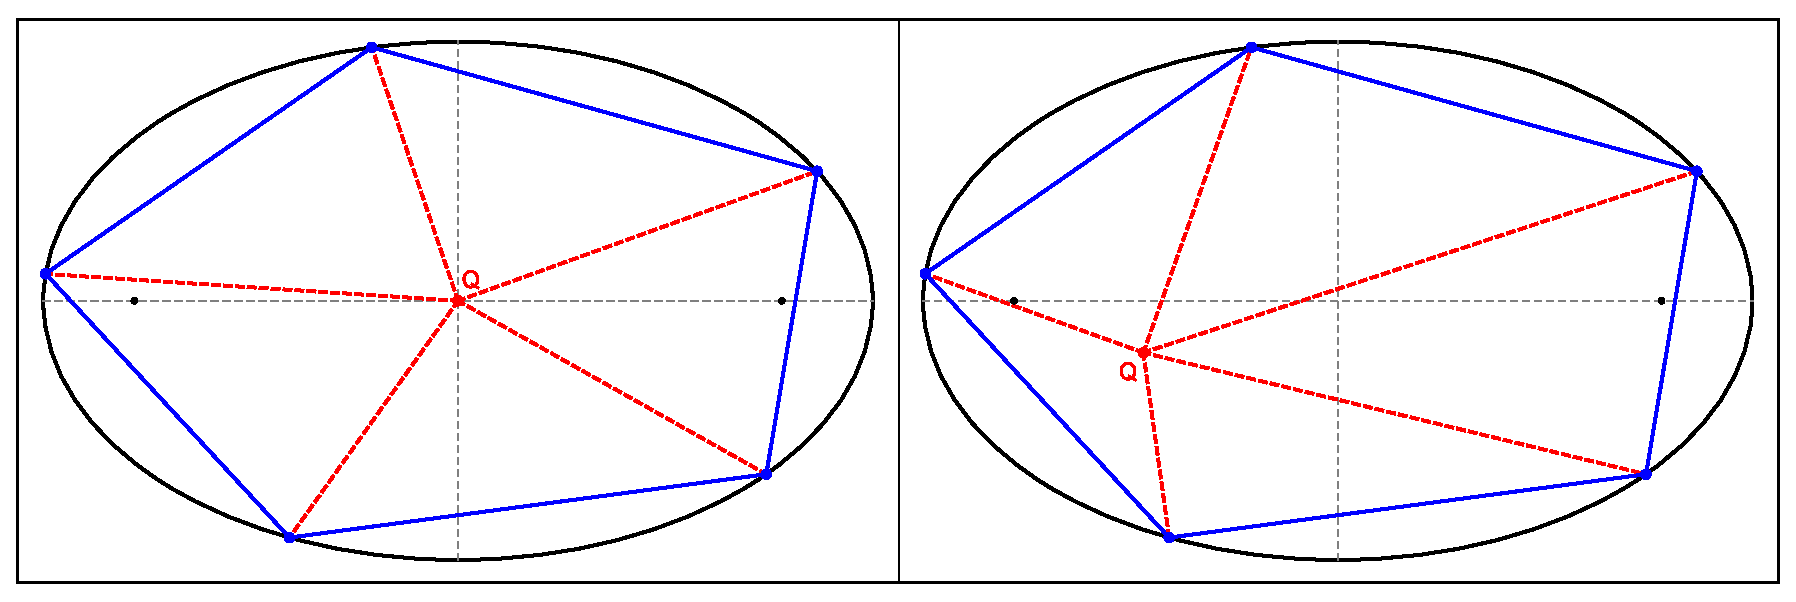
\includegraphics[width=\textwidth]{pics/0025_homot_norm_no_caustic.eps}
    \caption{\textbf{Left:} \cref{:norm2} states that the sum of squared norms of the vertices with respect to the center is invariant. \textbf{Right:} \cref{:p0} states that in fact the squared norms of vertices with respect to any point $P_0$ is invariant. \href{https://youtu.be/2PdsC3CcqaE}{Video}}.
    \label{fig:homot_norm}
\end{figure}

\begin{proof}
Apply \cref{:Laurent} with $f=(ax)^2+(by)^2$.
\end{proof}
\begin{remark}
For quadrangles this is known as
\href{https://en.wikipedia.org/wiki/Ellipse#Theorem_of_Apollonios_on_conjugate_diameters}{Theorem of Apollonios on conjugate diameters}.
\end{remark}

Let $s=|S(ρ(P)-P)|$ denote the sidelength,
then the trace $L_{2,N} := T_N s^2$ is a constant equal to
\begin{equation}
\label{:sqr_si}
T_N s^2 = \left[ 1-\cos \left(α\right) \right] \left( a^2+b^2 \right)
\end{equation}
\begin{proof}
Note that any rotation $ρ$ is linear, so coordinates of $ρ(P)-P$ are linear in $x,y$
and its scalar square is quadratic. Apply \cref{:Laurent}.
\end{proof}

Recall the Brocard angle $\omega$ of a triangle is given by $\cot\omega=L_{2,3}/(4A_3)$ \cite[Brocard Angle]{mw}. Then:

\begin{corollary}
Over $\FF$ with $N=3$, the Brocard angle $\omega$ is constant. 
\end{corollary}

Note: a well-known identity is that $\cot\omega=\cot\theta_1+\cot\theta_2+\cot\theta_3$.
\cref{:cot} is statement that this sum generalizes for $N>3$. 


Referring to \cref{fig:homot_norm}, the trace of the squared distance to any fixed point $Q$ is also constant:

\begin{equation}
\label{:p0}
T_N |P_k-Q|^2 = \frac{a^2 + b^2}{2} + |Q|^2
\end{equation}




\subsection{Cotangents}
\label{sec:cot}
The cotangent $\cot\theta$ is quadratic,
hence for $N>2$ its trace $T_N (\cot\theta)$ is a constant, it equals to
\begin{equation}
\label{:cot}
T_N \cot\theta = - \cot\left(α\right) \cdot \frac{\left( {a}^{2}+{b}^{2} \right) }{2ab}
\end{equation}
\begin{proof}
A cotangent is a ratio $\cot = \frac{Scalar}{Area}$ of a scalar product by an area.
Since an area is constant, a cotangent is quadratic iff a scalar product is quadratic.
The latter was established in the previous section. The projection formula relates the two traces. 
\end{proof}

\begin{corollary}
For $N>2M\geq0$
the traces $T_N (\cot^M(θ))$ of the powers of the cotangent are constants equal to the respective integrals.
\end{corollary}
\begin{proof}
Since the cotangent $\cot θ(\varphi)$ is a quadratic function
and its powers $\cot^M θ(\varphi)$ are polynomials of degree at most $2M$.
\Cref{:Laurent} implies that
the trace $T_N (\cot^M(θ))$ is constant for $N > 2M \geq 0$.
\end{proof}

% \begin{equation}
%  4\left(1-\cos\left(\frac{2\pi}{n}\right) \right)A_n Cot_n+ n\cos\left(\frac{2\pi}{n}\right) L_n = 0
% \end{equation}

The following explicit expressions for the sum of squared cotangents for $N>4$ can be derived.
\newcommand{\cN}{\cos\left(\frac{α}{2}\right)}
\newcommand{\sN}{\sin\left(\frac{α}{2}\right)}
\begin{equation}
\begin{aligned}
T_N \cot^2θ 
 = & -\frac{(a^2+b^2)^2\cos(2α)+2 (a^4+ b^4)}{ 4 (\cos(2α)-1) a^2 b^2 } \\
% = &\frac { -\left( {a}^{2}+{b}^{2} \right) ^{2} \sin^2(α) + \frac32\,{a}^{4}+{a}^{2}{b}^{2}+\frac32\,{b}^{4} }{4 {a}^{2}{b}^{2} \sin^2(α)}\\
 = &  \frac{3\,a^{4}+2\,a^{2}b^{2}+3\,b^{4}}{2\left( a^{2}+b^{2} \right)^{2}}
      \cdot \left(T_N\cotθ\right)^2
    + \frac{ \left(a^2-b^2 \right)^{2} }{8a^{2}b^{2}}
\end{aligned}
\end{equation} 

\begin{equation}
\lim_{α\to 0} α T_N   \cotθ    = -\frac{a^2+b^2}{2 ab},\;\;\;
\lim_{α\to 0} α^2 T_N \cot^2θ  =  \frac{3 a^4+2 a^2 b^2 +3 b^4}{ 8 a^2b^2  } 
\end{equation}


\subsection{Distances to a Focus, and the Curvature}
\label{sec:focuspocus}
Referring to \cref{fig:spoke-sum}, let $d_\pm$ denote the distance to the focus $f_\pm$ of $\EE$.

Given a point $P=(x,y)\in\EE$ and foci $F_\pm = (\mp c,0)$.
it is elementary to observe
\footnote{See \href{https://en.wikipedia.org/wiki/Ellipse\#Standard_equation}{Ellipse Standard Equation} on Wikipedia, namely: ``The distances from a point $(x,y)$ on the ellipse to the left and right foci are $a+ex$ and $a-ex$''.}
that these distances are linear polynomials
\begin{equation}
\label{eq:foci}
 d_+(P) = a + \frac{cx}{a}, \;\; d_-(P) = a - \frac{cx}{a}
\end{equation}

Thus over $\FF$ their traces are equal to $a$:
\begin{equation}
\label{:dist-focus}
T_N d_+ = T_N d_- = a
\end{equation} 

The curvature $κ(z)$ for a parametrized curve
\begin{equation*}
z\mapsto Z(z) = X(z) + Y(z)\cdot i
\end{equation*}
on a Cartesian Euclidean plane is given\footnote{See \href{https://en.wikipedia.org/wiki/Osculating_circle\#Mathematical_description}{Osculating Circle} on Wikipedia.}
in terms of the first two derivarives $Z',Z''$ 
\begin{equation}
\label{eq:curvature-parametrized}
κ = \frac{Area(Z',Z'')}{|Z'|^3},
\end{equation}

This formula does not depend on the choice of the coordinate
and it is convenient to use derivation with respect to $\log z$
\begin{equation}
W' := z\cdot \frac{\partial W}{\partial z}
\end{equation}
because it preserves the degree: if $Z(z)$ is a Laurent polynomial of degree $d$ then so are $Z'$ and $Z''$,
thus $|Z'|^2 = (Z',Z')$  and $Area(Z',Z'')$ are Laurent polynomials of degree at most $2d$.
Elevating \eqref{eq:curvature-parametrized} to the power $-2/3$ one obtains
\begin{equation}
\label{eq:curvature23-parametrized}
κ^{-2/3} = |Z'|^2 \cdot {Area(Z',Z'')}^{-2/3},
\end{equation}
so for any Laurent polynomial $Z$ the power $κ^{-2/3}$ is a Laurent polynomial
if and only if $Area(Z',Z'')$ is a perfect cube.
For a conic $\deg_z Z = 1$, so $Area(Z',Z'')$ is constant (degree $0$) in $z$.

{\color{orange} Comment this block, but do some experiments first.
For higher degree $d$ Area(Z',Z'') to be a perfect cube seems an unlikely condition.
Explicitly using $z^n \wedge z^m = \frac{z^{n-m} - z^{m-n}}2$
we have for $Z = \sum_{k=-d}^d c(k) z^k$
\begin{equation}
2i \cdot Z' \wedge Z'' = \sum_{n,m=-d}^d c(n)\cdot c(m)^2\cdot \left( z^{n-m}-z^{m-n} \right)
\end{equation}
}

In terms of semi-axes and distances to the foci of the ellipse, the curvature is 
$κ = (a b)\cdot (d_+ d_-)^{-3/2}$,
so the factorization \eqref{eq:curvature23-parametrized} takes the form
\begin{equation}
κ^{-2/3} = \left(d_+ d_-\right) \cdot \left(a b)\right)^{-2/3}.
\end{equation}
Note that $d_\pm$ are degree one by \eqref{eq:foci}.

It follows that $κ^{-2/3}$ is a quadratic polynomial over $\FF$ and for $N>2$ its trace is given by
\begin{equation}
\label{:kappa}
T_N \left(\frac{ab}{κ^2}\right)^\frac{1}{3} = \frac{a^2 + b^2}{2ab}
\end{equation}

\begin{figure}
    \centering
    \includegraphics[width=.6\textwidth]{pics/0060_spoke_sum.eps}
    \caption{Over the affinely-regular family, the sum of distances $d_+(P_i)=|P_i-f_+|$ is constant, where $f_+$ is a focus of the outer ellipse.}
    \label{fig:spoke-sum}
\end{figure}


\subsection{Evolute Polygon}
\label{sec:evolute}
Referring to \cref{fig:ev-poly-n5}, for a point  $P\in\EE$ 
define $\PP_u = P + u (C-P)$, where $u$ is a scalar and
$C$ is the center of the curvature
(i.e. the center of the circle osculating $\EE$ in $P$).
For fixed $u$ the map $P\mapsto \PP_u$ sends $\EE$
to the ``evolute curve'' $\EE_u$,
e.g. if $\EE_0 = \EE$ and $\EE_1$ is the evolute (i.e. the curve swapped by the centers of curvature).
Similarly vertices of the ``evolute polygons'' are defined as the images of
the vertices of affine-regular polygons.

Over $\FF$, the area $\AA_u$ of $\PP_u$ is constant, for all $N{\neq}1,2,4$. It is given by:
\begin{equation}
\small
\label{:as}
\frac{\AA_u}{N} = \frac{1}{32 a b}
\left[{{\left((a^2 + 3\,b^2)\cdot u- 4\,a^2 \right)
\left( (3\,a^2+b^2)\cdot u - 4\,b^2 \right) } \sin(α) }
+  u^2 c^4 \cdot \sin(3α)\right]
\end{equation}
 
\begin{proof}
The coordinates of $C$ (and hence of $\PP_u$)
are cubic trigonometric polynomials, odd with respect to the total grading.
{\color{red} In initial sections I have not described the total grading,
described only another one, that we do not really use.}
Therefore the area $A_u(P) = \frac{\PP_u\wedge \mathcal{ρ(P)}_u}2$
is an even Laurent polynomial of degree at most $6$.
In fact the highest degree terms of $\PP_u$ and $\mathcal{ρ(P)}_u$
are proportional, so $A_u(P)$ is an even Laurent polynomial of degree $4$.
Apply \cref{:Laurent} and compute $\AA_u := T_0 A_u$.
\end{proof}

\noindent The variation of $\AA_u$ for quadrangles is illustrated in \cref{fig:ev-poly-n4}.

\begin{corollary}
For every $N$ there are two values of $u$ such that $\AA_u = 0$.
\end{corollary}
\begin{proof}
\cref{:as} is quadratic in $u$: by definition $\PP_u$ and $\mathcal{ρ(P)}_u$
are linear in $u$ and wedge product is bilinear.
\end{proof}

\noindent \cref{fig:ev-poly-zero-area} illustrates null $\AA_u$ for $N\leq7$.
Referring to \cref{fig:zero-n3}:

\begin{observation}
%For the $N=3$ case, the area of $\AA_s$ is given by:
%\[{\frac { \sqrt {3} \left( 9\,{a}^{2}+3\,{b}^{2} \right) \left( {a}^{2}+3\,{b}^{2} \right) {u}^{2}}{64\,a\, b}}-{\frac {\sqrt {3} \left( 9\,{a}^{4}+6\,{b}^{2}{a}^{2}+9\,{b}^{4} \right) u}{16\,a \,b}}+{\frac {3\,\sqrt {3}\; a b}{4}}\]
For triangles, $\AA_u=0$ for $u=4b^2/(3a^2 + b^2)$ or $u=4a^2/(a^2 + 3b^2)$;
in each case, the vertices of $\PP_u$ are collinear and parallel to the axes of either ellipse.
\end{observation}

Indeed, as shown on this \href{https://youtu.be/OFA_j25R8ks}{Video}, these two segments meet at the {\em 3rd Brocard point} of the triangle \cite[X(76)]{etc}.

\begin{observation}
Only for triangles and quadrangles, the family of $\PP_u$ has constant sum of cotangents, for all $u$.
Note that for triangles this sum is not defined if $\AA_u=0$ (a segment has $3$ null angles);
for quadrangles said sum is equal to zero (family of parallelograms).
\end{observation}

Referring to \cref{fig:zero-area-inf}, when $Ν{\rightarrow}\infty$ (more generally, $α\rightarrow 0$ or $ζ\rightarrow 1$),
\begin{equation}
\label{eqn:ninf}
\lim_{α\to 0}
\frac{\AA_u}{πab} = 1 - \frac {\, \left( 3\,{a}^{4}+2\,{a}^{2}{b}^{2}+3\,{b}^{4} \right)}{8\,a^2\, b^2} \cdot u (2-u).
\end{equation}
%\textcolor{red}{ronaldo $\AA_s=...$ at $u=...$. These curves are known as ... or have degree ...}.

\begin{figure}
    \centering
    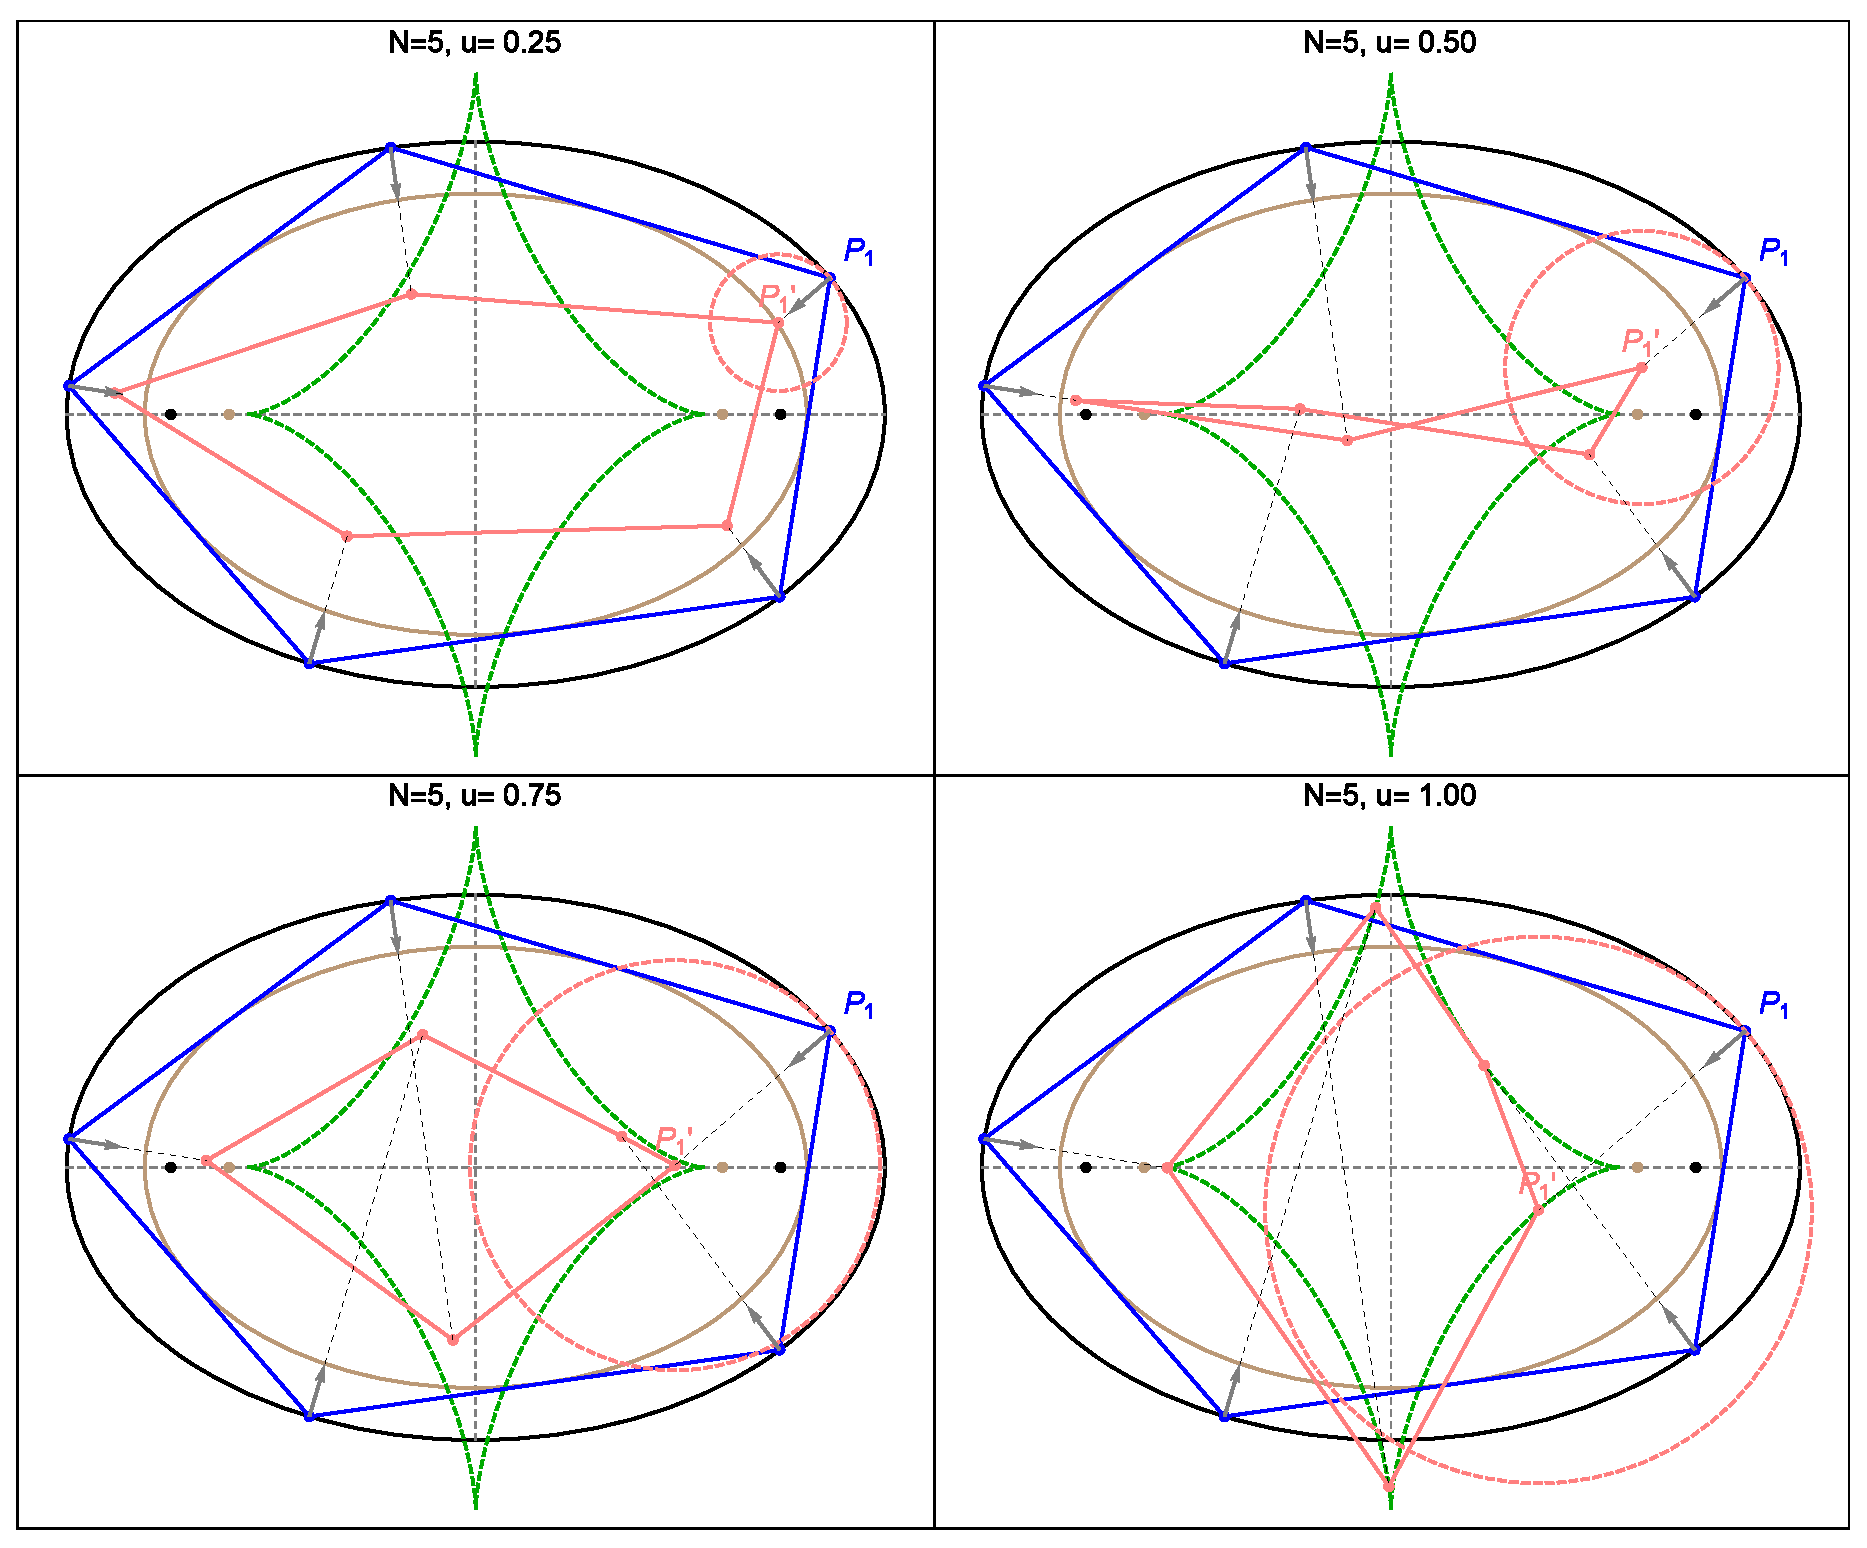
\includegraphics[width=\textwidth]{pics/0070_evolute_poly_n5.eps}
    \caption{Constant signed-area evolute pentagons (pink) for various values of $u$. The outer ellipse has $a/b=3/2$. The dashed circle centered on $P_1'$ and passing through $P_1$ has radius $u R_1$ where $R_1$ is the inverse curvature at $P_1$. Notice that when $u=1$ (bottom right), the $P_i'$ lie on the evolute (dashed green). \href{https://youtu.be/JCj0q7_hlA8}{Video}}
    \label{fig:ev-poly-n5}
\end{figure}

\begin{figure}
    \centering
    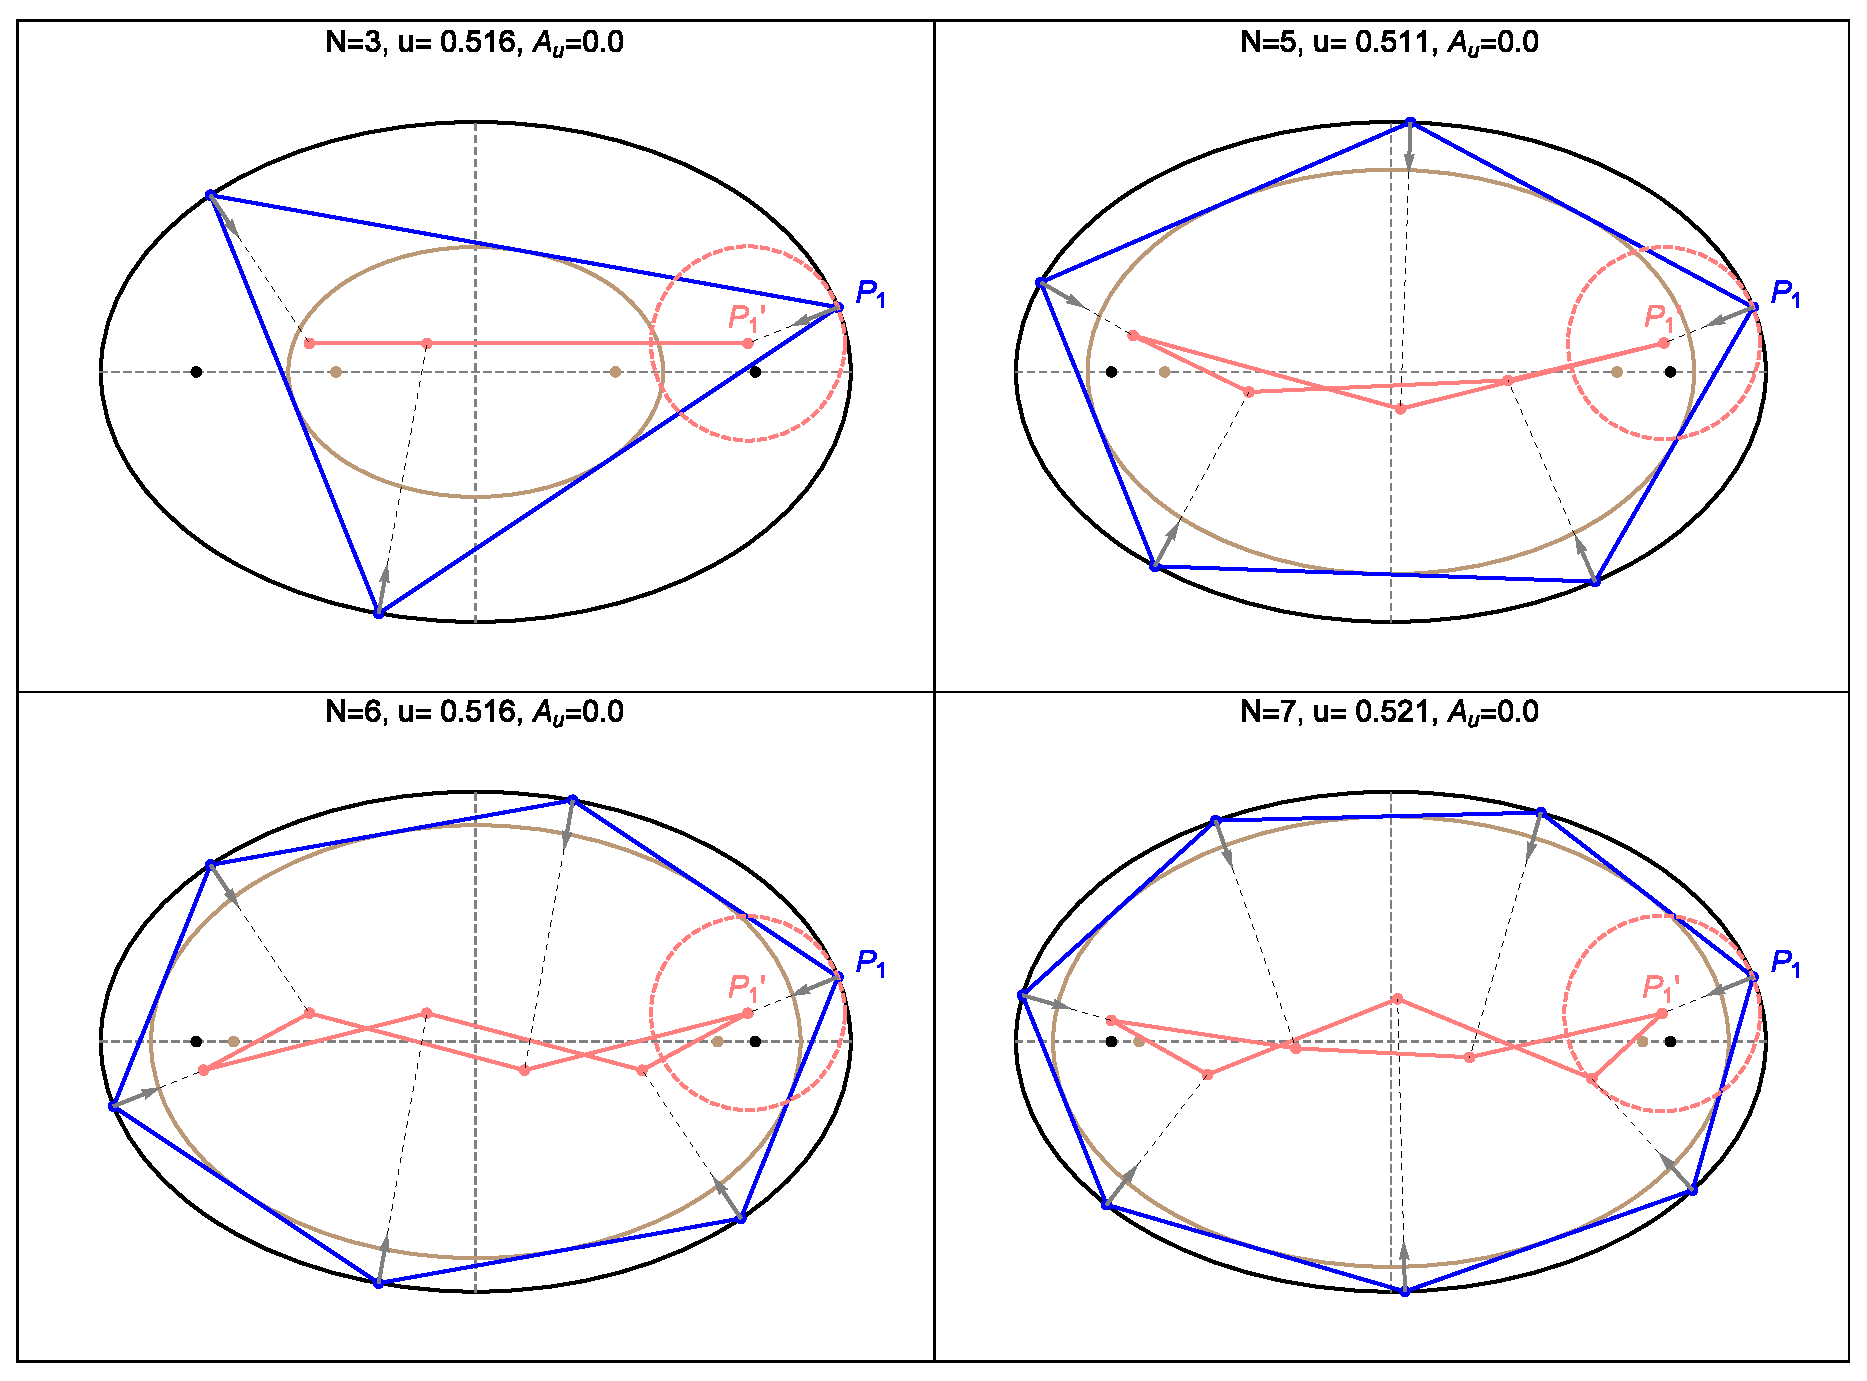
\includegraphics[width=\textwidth]{pics/0080_evolute_poly_zero_area.eps}
    \caption{Zero-area evolute triangles, pentagons, hexagons and septagons (pin) inscribed in an ellipse with $a/b = 3/2$.
             Quadrangles are omitted as for all $u$, its area is variable. \href{https://youtu.be/3nvXYFoI5Wg}{Video}.}
    \label{fig:ev-poly-zero-area}
\end{figure}

\begin{figure}
    \centering
    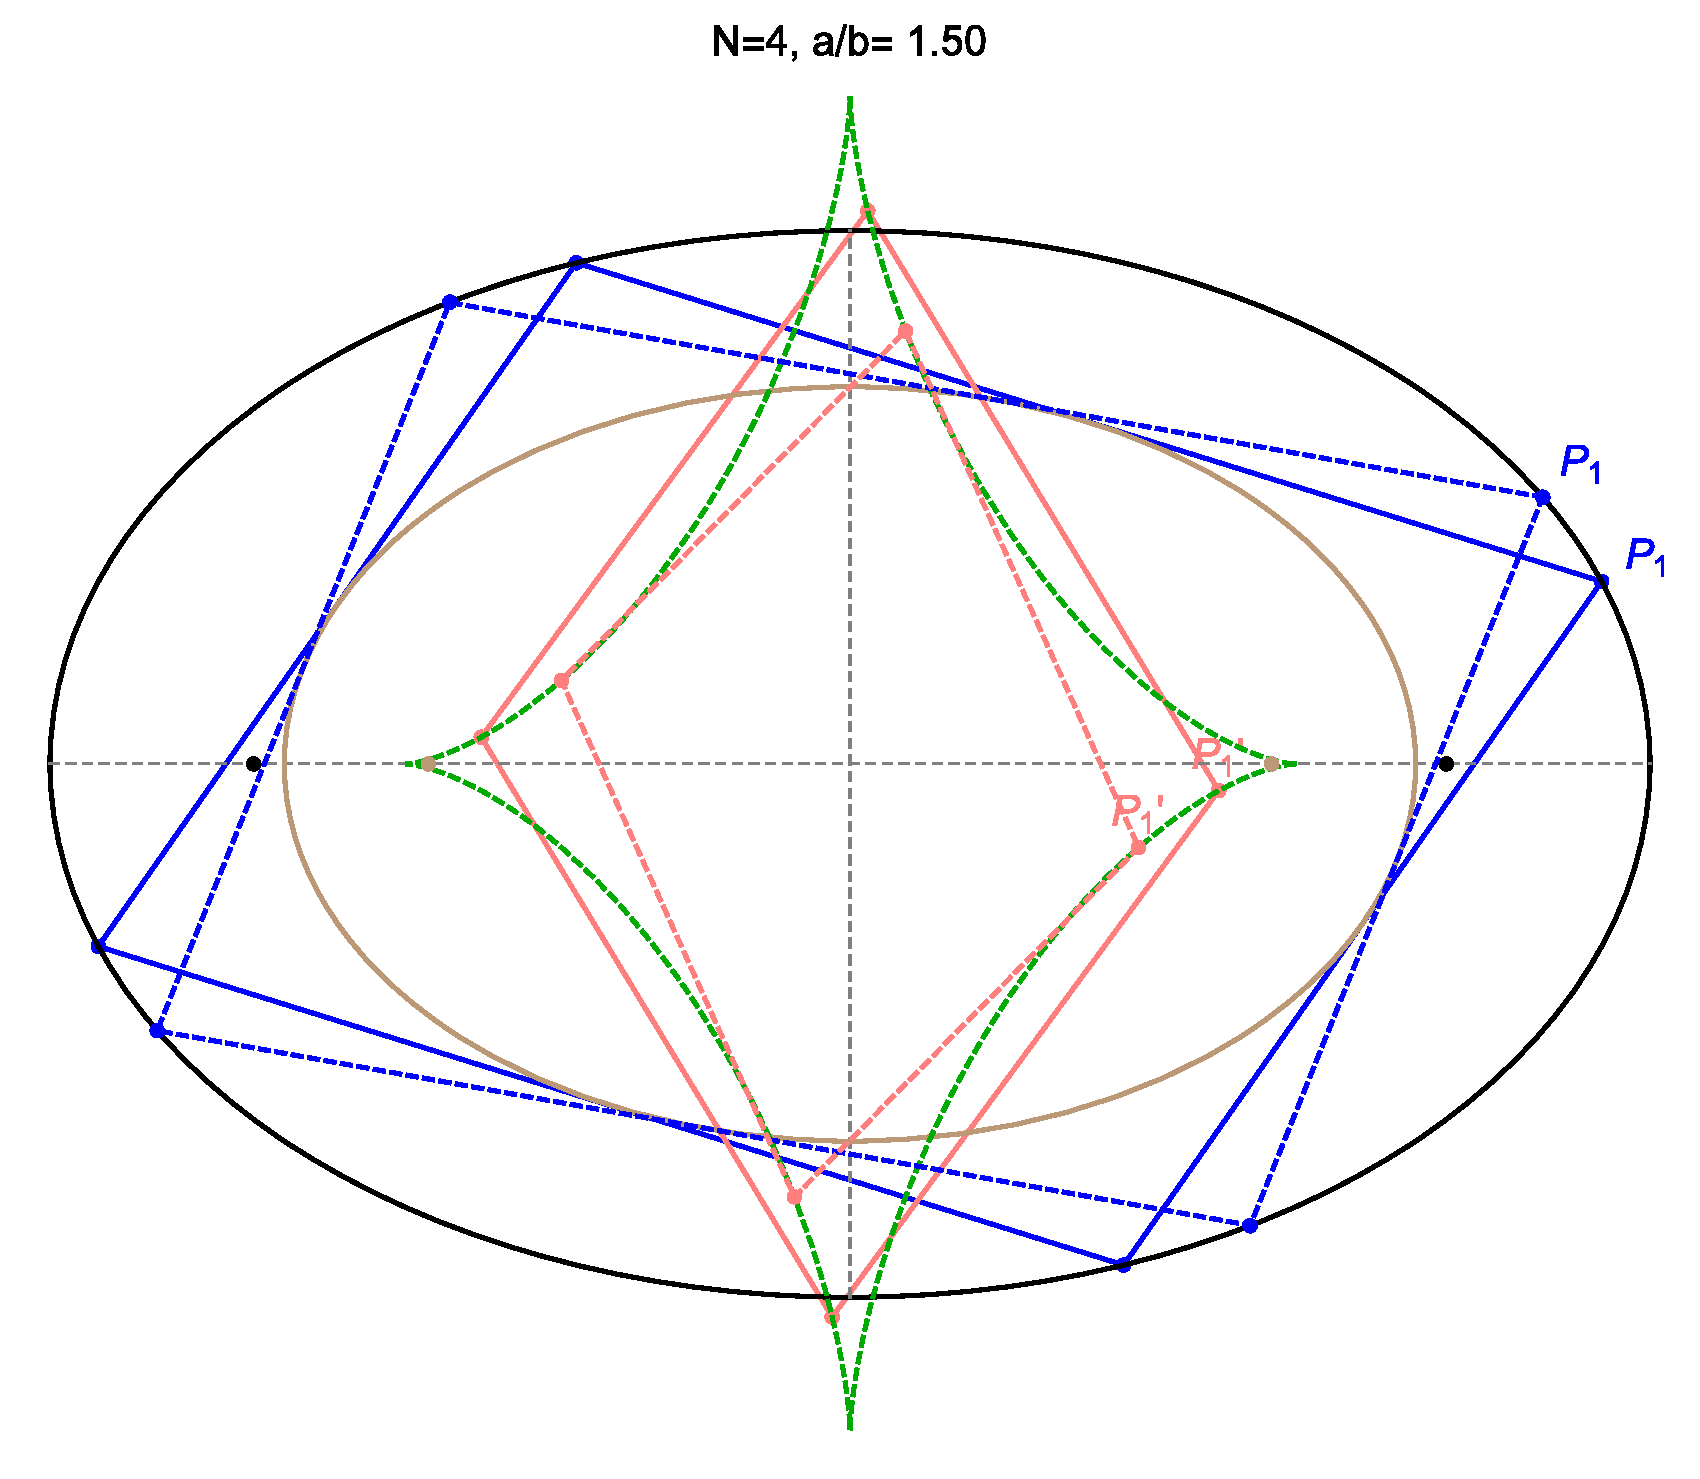
\includegraphics[width=.7\textwidth]{pics/0050_n4_ev_poly.eps}
    \caption{Two quadrangles (blue and dashed blue) and their respective evolute polygons $\PP_u$ (pink, dashed pink), for $u=1$.
             Exclusively for quadrangles, $\AA_u$ is variable, for any $u$ chosen.
             Note that the $T_N u^2$ is variable for both quadrangles and hexagons.
             {\color{red} If variables for hexagons shall be variable for triangles as well, cf \cref{:functoriality}.}
             }
    \label{fig:ev-poly-n4}
\end{figure}


\begin{figure}
    \centering
    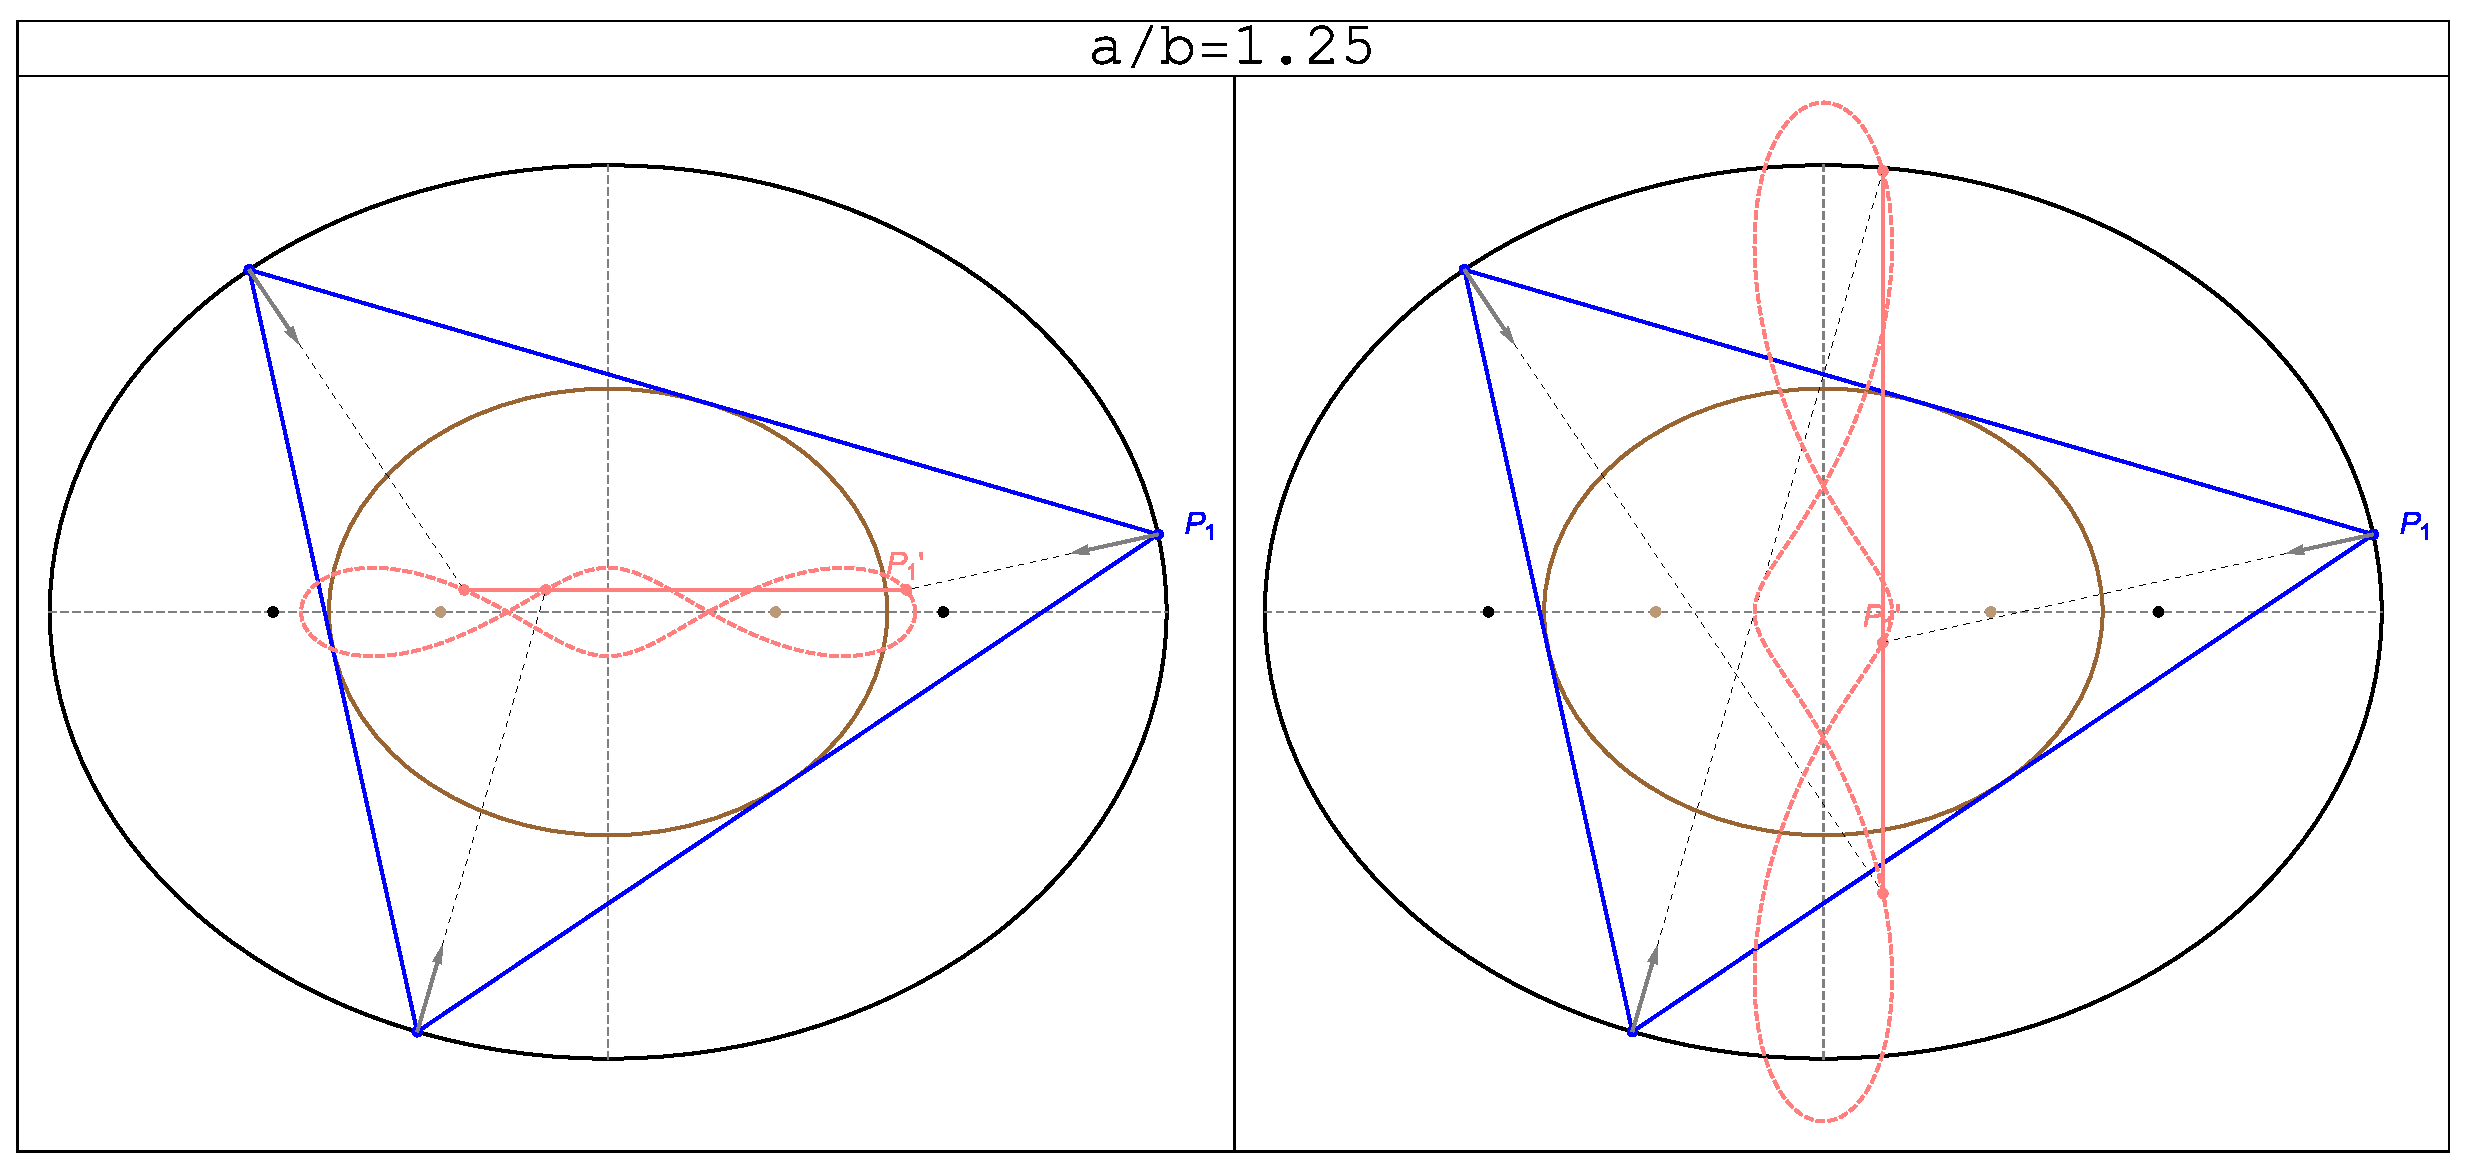
\includegraphics[width=\textwidth]{pics/0090_zero_area_n3_both.eps}
    \caption{The two zero-area evolute triangles are segments parallel to either axes of the ellipses.
             Also shown is the self-intersected locus of their vertices. \href{https://youtu.be/f80QaYs5_J4}{Video 1}.
             It turns out the two segments meet at the triangle center named $X_{76}$ \cite{etc} \href{https://youtu.be/OFA_j25R8ks}{Video2}.}
    \label{fig:zero-n3}
\end{figure}

\begin{figure}
    \centering
    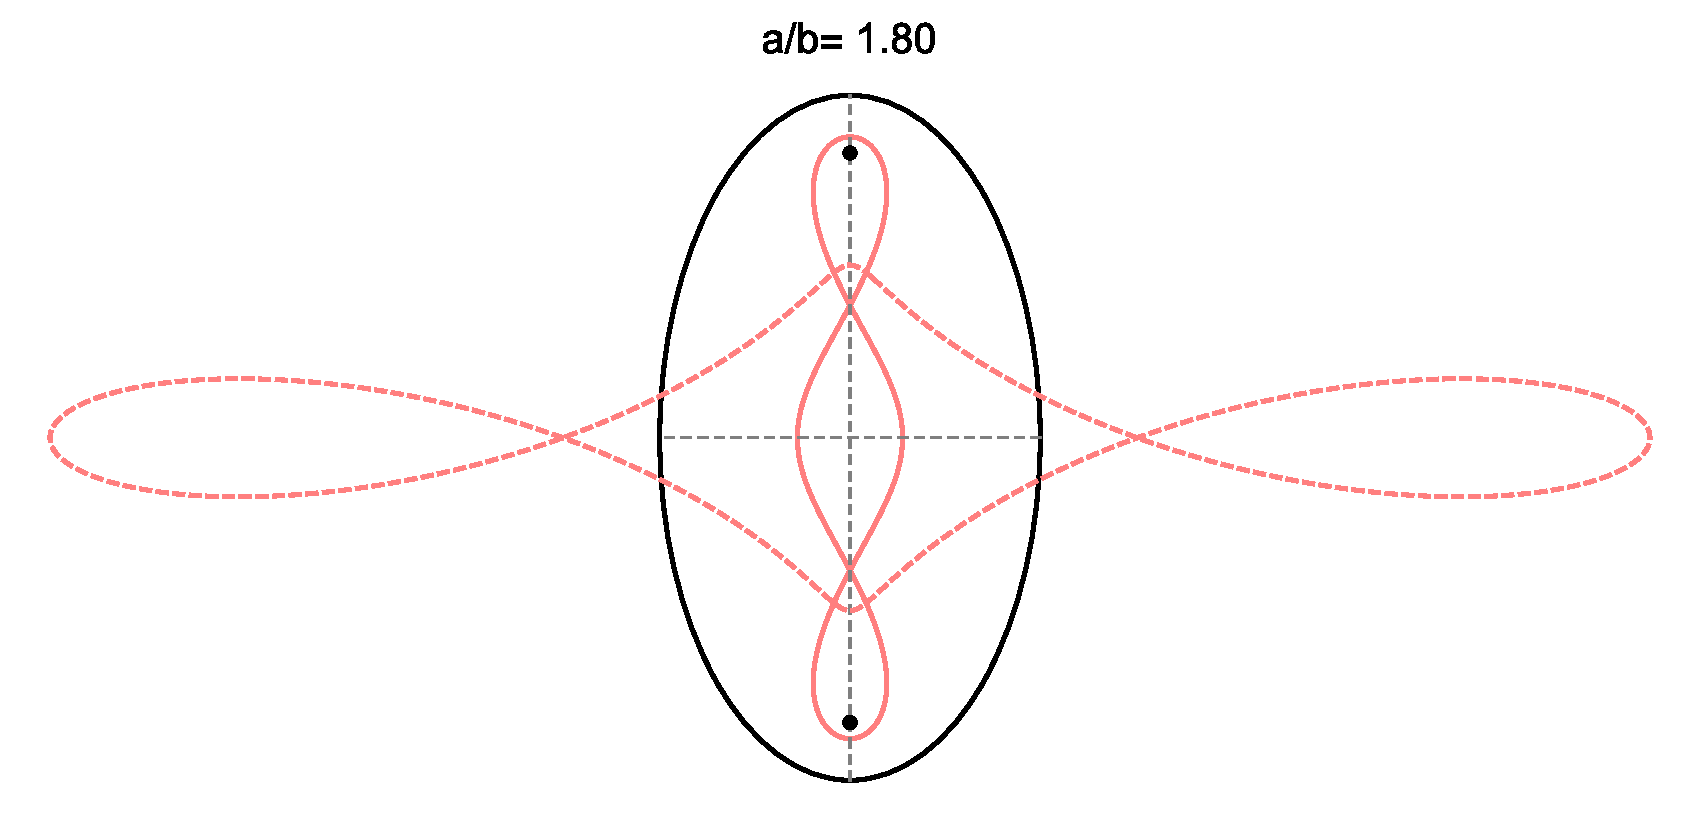
\includegraphics[width=.7\textwidth]{pics/0100_zero_area_ninf_both.eps}
    \caption{The two zero-area evolute polygons (pink and dashed pink) when $N$ is infinite, see \cref{eqn:ninf}.}
    \label{fig:zero-area-inf}
\end{figure}

Note when $u=0$, $\PP_u$ is the original polygon, and the sum of its squared sidelengths is a constant given in \cref{:sqr_si}.

Let $\ell_i$ denote the $i$-th sidelength of $\PP_u$.

If $s{\neq}0$ and $N{\notin}\{1,2,3,4,6\}$, the trace $T_N \ell^2$ is a constant equal to:
{\small  
\begin{equation}
\label{:ell2}
 2 \sin^2\left(\frac{α}{2}\right) \left[ \frac{c^4 u^2}{2}\left ( \cos α \cos^2\left(\frac{α}{2}\right) \right) +\frac{u^2}{8}( 5a^4  - 2a^2b^2  +  5b^4 )  - a^2b^2(2 u - 1)\right] \frac{ a^2+b^2}{a^2 b^2}
\end{equation}

\begin{equation}\aligned
 & - \,{\frac {{u}^{2} \left( {a}^{2}-{b}^{2} \right) ^{2} \left( {a}^
{2}+{b}^{2} \right) }{16{a}^{2}{b}^{2}}}\cos 3\alpha\\
&-\left( \,{\frac { \left( 9\,{a}^{4}-2\,{a}^{2}{b}^{2}+9\,{b}^{4}
 \right)  \left( {a}^{2}+{b}^{2} \right) {u}^{2}}{16{a}^{2}{b}^{2}}}+
 \left( {a}^{2}+{b}^{2} \right)  \left( 1-2\,u \right) 
\right)\cos\alpha\\
&+\frac { \left( 5\,{a}^{4}-2\,{a}^{2}{b}^{2}+5\,{b}^{4} \right) 
 \left( {a}^{2}+{b}^{2} \right) {u}^{2}}{8{a}^{2}{b}^{2}}+ \left( {a}^
{2}+{b}^{2} \right)  \left( 1-2\,u \right) 
\endaligned
\end{equation}

%\textcolor{green}{ron: done}
%{\color{red} Simplify the formula. All entities like $\sin^2(α/2)$, $\cos^2(α/2)$ can be given in terms of $\sin(α)$, $\cos(α)$.
%Compare with the script that computes everything in terms of powers of $ζ$(named $w$),
%i.e. in terms of $\cos(nα)$ and $\sin(nα)$ with $n$ integer. }
}
\begin{proof}
Similar to the case of \cref{:as}, but without cancellation of the leading terms,
so $\ell^2$ is an even trigonometric polynomial of degree six with non-vanishing
fourth coefficient, the cases $N=1,2,3$ are impossible thanks to \cref{:functoriality}. %Note that for $N=3$ the quantity isn't constant because $N\neq 6$ implies $N\neq3$.
\end{proof}


\section{Affine Image of a Regular Polygon}
 

%\section{Affine image of a regular polygon}

Consider the regular $N$-gon with vertices given by 
\[ Q_k=(\cos\frac{2k\pi}{N},\sin\frac{2k\pi}{N})= (\cos k\alpha,\sin k\alpha)\]
and the affine map $T$
%$T(x,y)=(ax+py,qx+by)$
defined by the matrix 
$\begin{pmatrix}a&p\\q&b\end{pmatrix}$.  % [a,p;q,b]

Let $v_1=(a,q)$,  $v_2=(p,b)$.  Write 
 $v_1\wedge v_2=ab-pq=\Delta$ and $\langle v_1,v_2\rangle =aq+bp=\Rho$.



Then,  the  polygon $\PP$ with vertices
$P_k=TQ_k$ has the following properties:



\begin{align*}
  \frac1{N} A(\PP) &= \sin\alpha \Delta  \\
  \frac1{N} \sum |P_k|^2   &= \frac{1}{2}(|v_1|^2+ |v_2|^2 )\\
    \frac1{N} \sum |P_{k+1}-P_k|^2   &=(1-\cos\alpha)(|v_1|^2+|v_2|^2)\\
  \frac1{N}  cot_N  = \frac1{N}  \sum \cot_k &= -\frac{1}{2}\cot\alpha \frac{|v_1|^2+ |v_2|^2}{\Delta}\\
   &=-\cos\alpha \frac{\sum |P_k|^2}{A(\QQ)}
\end{align*}
   
 Also,
 
 \begin{align*}
  \frac{1}{N} \sum\cot_k^2& = \frac{ \left(   |v_1|^2+|v_2|^2 \right)^{2}
\cos \left( 2\,\alpha \right) +2\,  |v_1|^4
+4\, \Rho^{2}+2\, |v_2|^4
   }{8\, \Delta^{2}   \sin^2\alpha} \\
   &=\frac{ 2\left(   |v_1|^2+|v_2|^2 \right)^{2}
\cos^2  \alpha  + \,  |v_1|^4
+2(\Rho^2-\Delta^2) +\, |v_2|^4
   }{8\, \Delta^{2}   \sin^2\alpha
 }\end{align*}

Consider the evolute polygon $\PP_u$. Then it follows that

\begin{align*}
    \frac{1}{N}\AA_s &= \frac{1}{16\Delta} \left(A_1\sin\alpha +A_3\sin 3\alpha\right)\\
    A_1  &= (4\Delta^2 + 3|v_1|^4 + 3|v_2|^2 (2|v_1|^2 +|v_2|^2))u^2 \\
    &- (16\Rho^2 + 12|v_1|^4 + 4|v_2|^2(2|v_1|^2 + 3|v_2|^2))u + 16\Delta^2\\
    A_3 &= (|v_1|^4+2(\Rho^2-\Delta^2)+|v_2|^4)u^2
\end{align*}
\begin{align*}
   \frac{1}{N} \sum \ell_i^2&=\frac{|v_1|^2+|v_2|^2}{16\Delta^2}[B_3\cos 3\alpha+ B_1\cos\alpha+B_0]\\
    B_3 &=  (|v_1|^4+2(\Rho^2-\Delta^2)+|v_2|^4)u^2\\
    B_1 &=  (9|v_1|^4+2(9\Rho^2-\Delta^2)+9|v_2|^4)u^2+16(1-2 u)\Delta^2 \\
    B_0 &= -(10|v_1|^2-4\Delta^2+20\Rho^2+10|v_2|^4)u^2+16(2 u-1)\Delta^2
\end{align*}


%\section{Summary}

\begin{table}
\begin{tabular}{|l|l|l|l|l|l|}
\hline
id & system & outer conic & inner conic & \makecell[lt]{$N=3$\\invariants} & \makecell[lt]{$N>3$\\holds?} \\
\hline
0 & billiard & ellipse $(a,b)$ & confocal caustic & $L,J,r/R,\color{red}\sum\cos$ & $L,J,\color{red}\sum\cos$ \\
1 & inner circle & ellipse $(a,b)$ & circle $r=\frac{{a}{b}}{a+b}$ & $R,r/R,\color{red}\sum\cos$ & $\color{red}\sum\cos$ \\
2 & outer circle & $R=(a+b)$ & ellipse $(a,b)$ & $\sum{s_i^2},\color{red}\prod\cos$ & $\sum{s_i^2},\color{red}\prod\cos$ \\
\textbf{3} & \textbf{homothetic} & \textbf{ellipse $(a,b)$} & \textbf{ellipse $(a/k,b/k)$} & $A,\sum{s_i^2},\omega,\color{red}\sum\cot$ & $A,\sum{s_i^2},\color{red}\sum\cot$ \\
4 & $X_4$ stationary & ellipse $(a,b)$ & ellipse $(a_0,b_0)$ & $X_4=0$ & pseudo-$X_4$ = 0 \\
\hline
\end{tabular}
\end{table}

%\begin{figure}
%    \centering
%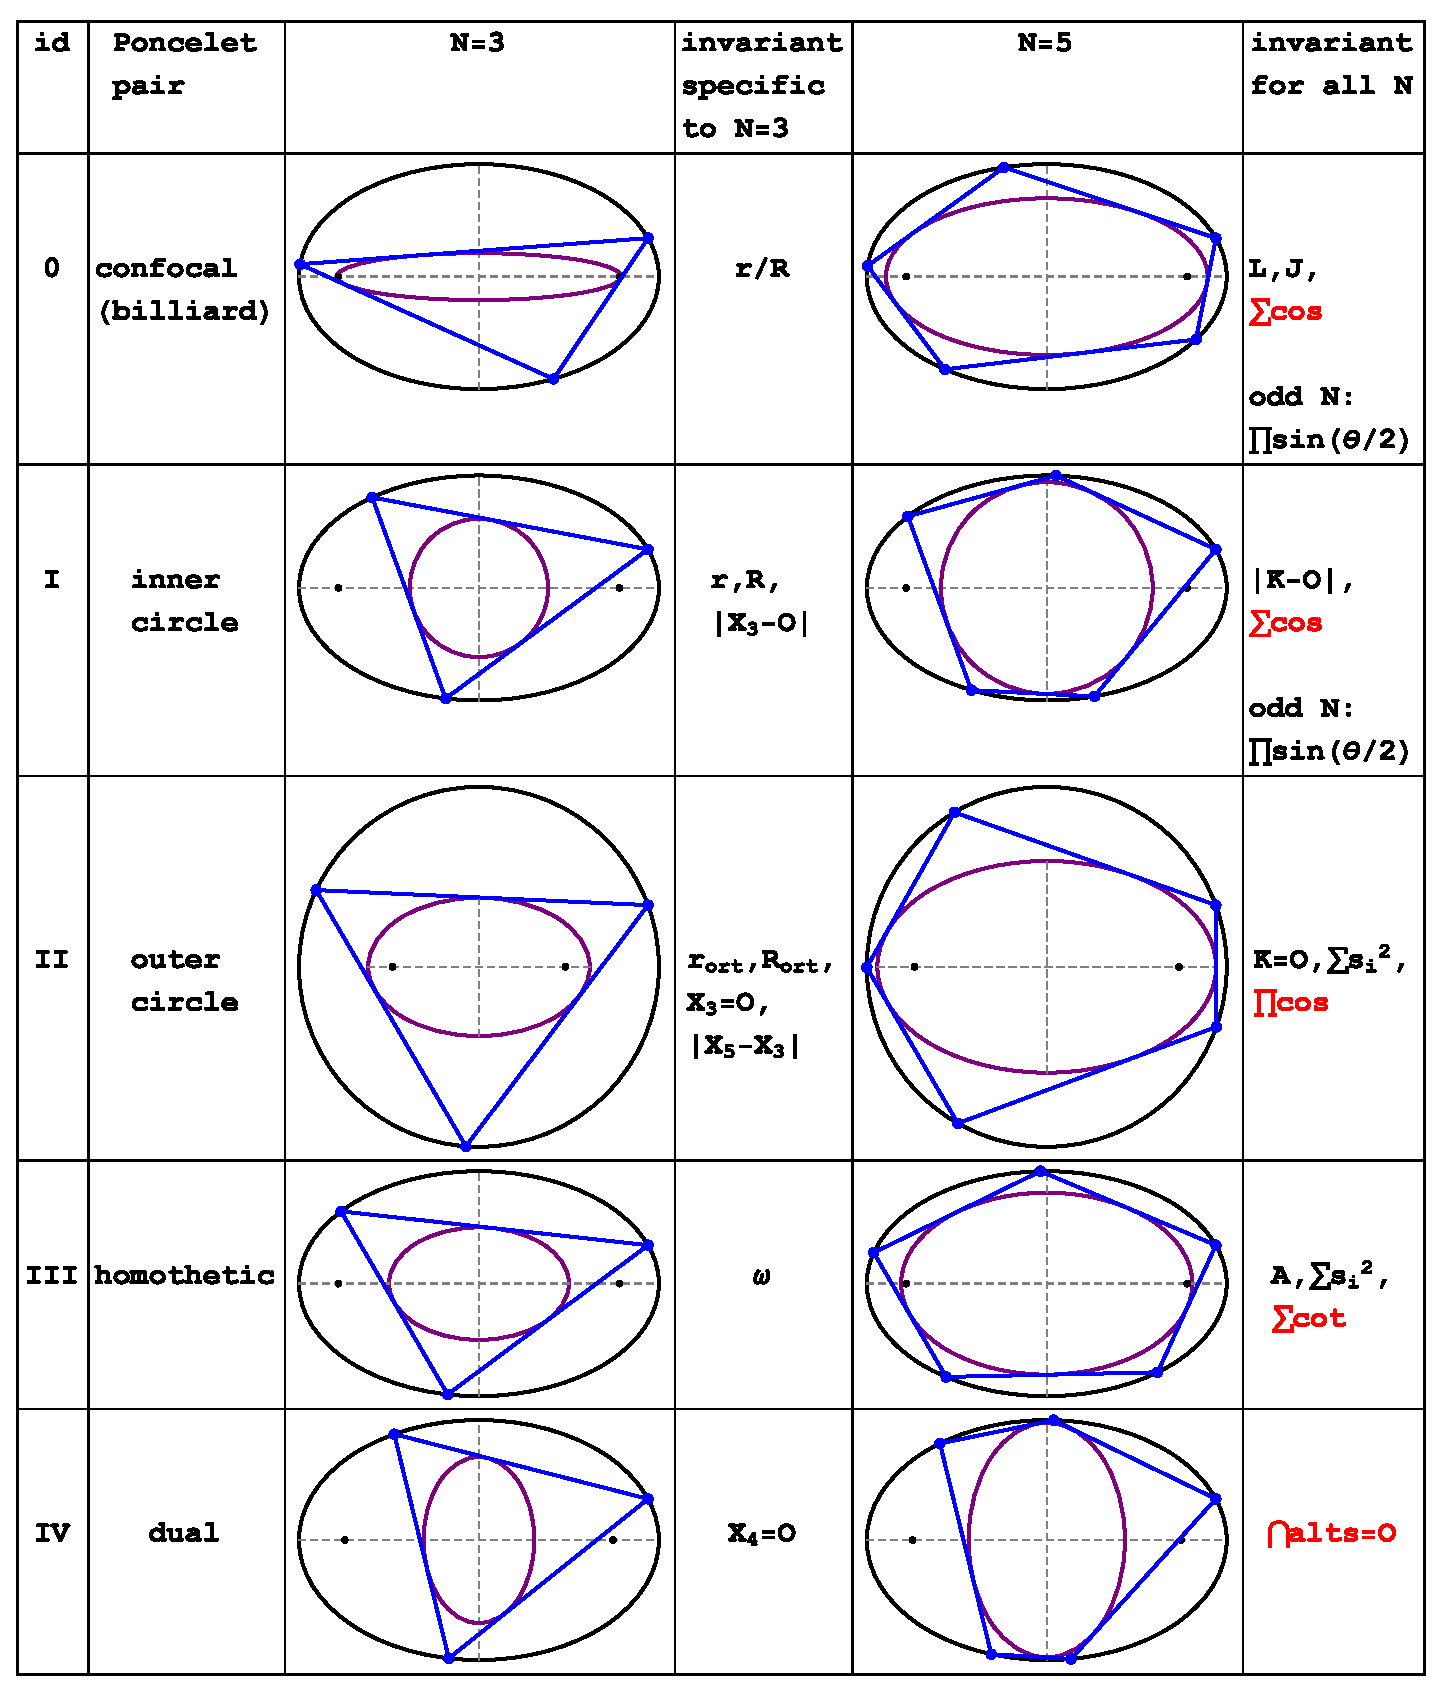
\includegraphics[width=\textwidth]{pics/0060_all_systems.eps}
%    \caption{}
%    \label{fig:all-systems}
%\end{figure}

\section{Summary and Videos}
\label{sec:video-table}

In \cref{tab:invariants-degrees} we summarize the quantities
that have constant trace with respect to $N$-isogenies.
On the left hand side we list polynomial quantities (and their degree),
such that their traces for the respective $N$-isogenies of genus zero curves (circles) are constant.
On the right hand side we list ``analogous'' quantities for the elliptic billiard,
such that their traces for the respective $N$-isogenies of genus-1 curves (Poncelet configuration spaces) are constant.

\newcommand{\mcc}[1]{\makecell[cc]{#1}}
\begin{table} 
\centering
\begin{tabular}{|c|c|c||c|c|} \hline
\mcc{degree} & \mcc{grading} & \mcc{polynomial\\quantity} & \mcc{confocal\\analogue} & \mcc{grading} \\ \hline
0 &  0  & $1$          & $1$               &   0  \\
0 &  1  & $a,b,c$      & --                &      \\
0 &  2  & $A$          & --                &      \\ \hline
1 &  1  & $d(P,f_\pm)$ & $d(P,f_\pm)^{-1}$ &  -1  \\ \hline
  & 2/3 & $κ^{-2/3}$   & $κ^{2/3}$         & -2/3 \\ 
2 &  0  & $\cotθ$      & $\cosθ$           &   0  \\
  &  2  & $s^2$        & $s$               &   1  \\
  &  2  & $d(P,P_0)^2$ & --                &      \\ \hline
4 &  2  & $\AA_s$      & --                &      \\ \hline
6 &  2  & $\ell^2$     & --                &      \\ \hline
\end{tabular}
\caption{Polynomial quantities on $\FF$ (homothetic pair of $N$-gons),
          their degree, and invariants in the confocal pair (elliptic billiard) which bear symbolic resemblance.
         The quantities $1,a,b,c,d(P,f_1),κ^{-2/3},d(P,P_0)^2$ are defined in terms of the ellipse $\EE$ alone,
         others also use the ellipse inscribed in the polygon.
}
\label{tab:invariants-degrees}
\end{table}

Animations illustrating some invariant phenomena herein are listed on Table~\ref{tab:playlist}.

\begin{table}[H]
\small
\begin{tabular}{|c|c|l|l|}
\hline
id & N & Title & \textbf{youtu.be/<.>}\\
\hline
01 & 5 & {Invariants of $\FF$} &
\href{https://youtu.be/2PdsC3CcqaE}{\texttt{2PdsC3CcqaE}}\\
02 & 3 & {Invariant Brocard Angles for triangles of $\FF$} & \href{https://youtu.be/2fvGd8wioZY}{\texttt{2fvGd8wioZY}} \\
03 & 3 & {Locus of Brocard Points for triangles of $\FF$} & \href{https://youtu.be/13i3JGY-fK4}{\texttt{13i3JGY-fK4}}\\
04 & 5 & {Invariant signed area of Evolute Polygon, $s=\{.25,.5,.75,.1\}$} & \href{https://youtu.be/JCj0q7_hlA8}{\texttt{JCj0q7\_hlA8}} \\
05 & 3,5,6,8 & {Evolute Polygons with Zero Signed Area} & \href{https://youtu.be/3nvXYFoI5Wg}{\texttt{3nvXYFoI5Wg}} \\
06 & 5 & {Invariant-Area Evolute Polygon with $s=1$} & \href{https://youtu.be/ChsfLzKrb4o}{\texttt{ChsfLzKrb4o}} \\
07 & 3 & {Zero-area Evolute Polygon is a horizontal segment} & \href{https://youtu.be/f80QaYs5_J4}{\texttt{f80QaYs5\_J4}} \\
08 & 3 & {Two zero-area evolute polygons intersect on $X_{76}$} & \href{https://youtu.be/OFA_j25R8ks}{\texttt{OFA\_j25R8ks}} \\
\hline
\end{tabular}
\caption{Illustrative videos. The last column is clickable and provides the YouTube code.}
\label{tab:playlist}
\end{table}



\section*{Acknowledgements}
\noindent We would like to thank S. Tabachnikov and A. Akopyan for valuable insights. The second author is fellow of CNPq and coordinator of Project PRONEX/ CNPq/ FAPEG 2017 10 26 7000 508.

\appendix

\section{Table of Symbols}
\begin{table}[H]
\small
\begin{tabular}{|c|l|l|}
\hline
symbol & meaning & note \\
\hline
$\EE,\EE_c$ & outer and inner homothetic ellipses & \\
$N$ & vertices of $N$-gon & \\
$O$ & center of concentric pair & \\
$a,b$ & semi-axes of $\EE$ & \\
$c$ & half the focal length of $\EE$ & $c^2=a^2-b^2$ \\
$a_c,b_c$ & semi-axes of $\EE_c$ & $(a_c,b_c) = \cos(\pi/N) (a,b)$ \\
$P_i,\theta_i$ & Poncelet vertices and angles & $i=1,...,N$\\
$f_\pm$ & foci of $\EE$ & $[\mp c,0]$ \\
$d_\pm(P)$ & distance from $P$ to $f_\pm$ & $|P-f_\pm|$ \\
$s_i$ & $i$-th sidelength & $|P_{i+1}-P_i|$, $i+1$ mod $N$\\
$A,L$ & area and perimeter & $\sum{s_i}$ \\
$L_{2}$ & sum of squared sidelengths & $\sum{s_i^2}$ \\
$\omega$ & Brocard angle ($N=3$) & $\cot\omega=L_{2}/(4A)=\sum\cot{\theta_i}$ \\
$\PP_u,\ell_i$ & evolute polygon and its $i$-th sidelength & \\
\hline
\end{tabular}
\caption{Symbols used.}
\label{tab:symbols}
\end{table}

\label{app:symbols}

\bibliographystyle{maa}
\bibliography{references,authors_rgk} 

\clearpage
 

\vskip 1cm
\address{ \noindent Sergey Galkin, \texttt{cotangent@galkin.org.ru} \\
Departamento de Matemática\\
% Pontifícia Universidade Católica do Rio de Janeiro - 
PUC-Rio\\
Rua Marquês de São Vicente 225, Gávea,
Rio de Janeiro, RJ, Brazil, 22451-900

 
\vskip .5cm
\noindent Ronaldo Garcia, \texttt{ragarcia@ufg.br} \\ 
 Instituto de Matemática e Estatística\\
Universidade Federal de Goiás\\
Goiânia, GO, Brazil, 74690-900

\vskip .5cm
\noindent Dan Reznik, \texttt{dreznik@gmail.com} \\ 
 Data Science Consulting\\
Rio de Janeiro, RJ, Brazil, 22290-240
}
 


\end{document}
